\documentclass[a4paper, 12pt, one column]{article}
%% Language and font encodings. This says how to do hyphenation on end of lines.
\usepackage[english]{babel}
\usepackage[utf8x]{inputenc}
\usepackage[T1]{fontenc}
%\usepackage{aas_macros}
\usepackage{parskip}

%% Sets page size and margins. You can edit this to your liking
\usepackage[top=1.3cm, bottom=2.0cm, outer=2.5cm, inner=2.5cm, heightrounded,
marginparwidth=1.5cm, marginparsep=0.4cm, margin=2.5cm]{geometry}

%% Useful packages
\usepackage{graphicx} %allows you to use jpg or png images. PDF is still recommended
\usepackage[colorlinks=True]{hyperref} % add links inside PDF files
\usepackage{amsmath}  % Math fonts
\usepackage{amsfonts} %
\usepackage{amssymb}  %
\usepackage{subcaption}
%% Citation package
\usepackage[authoryear]{natbib}
\usepackage{float}
\bibliographystyle{abbrvnat}
\setcitestyle{authoryear,open={(},close={)}}


\title{Project III: Protein Structures and Chimera}
\author{Lu Zhicong}

\begin{document}
\maketitle

\section{Exercise 1}
\subsection*{(a) Load the structure with ID 1HEW into Chimera.}
\begin{figure}[H]
    \centering
    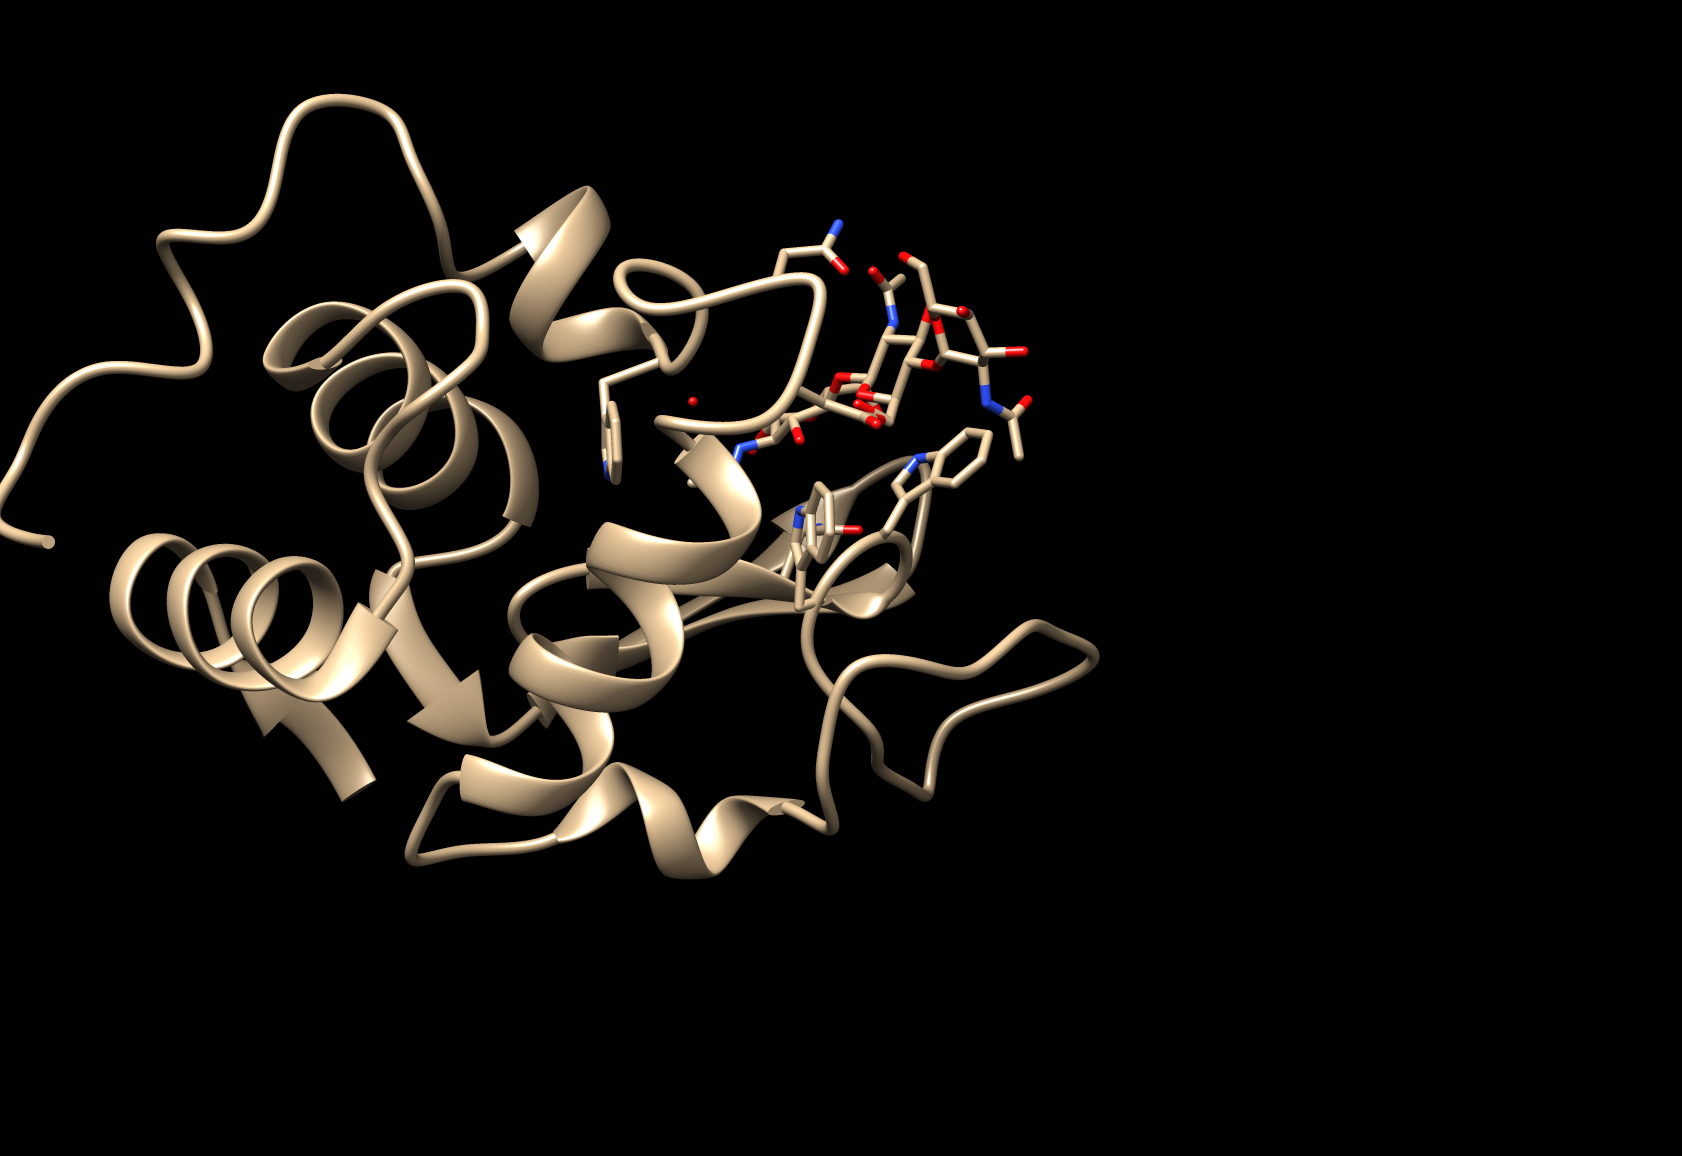
\includegraphics[width=.8\linewidth]{1_a.png}
    \caption{1.a}
    \label{fig:1_a.png}
\end{figure}
\subsection*{(b) What is this structure? Look for basic information.}
REFINEMENT OF AN ENZYME COMPLEX WITH INHIBITOR BOUND AT PARTIAL OCCUPANCY. HEN EGG-WHITE LYSOZYME AND TRI-N-ACETYLCHITOTRIOSE AT 1.75 ANGSTROMS RESOLUTION\\
PDB DOI: 10.2210/pdb1HEW/pdb\\
Classification: HYDROLASE(O-GLYCOSYL)\\
Organism(s): Gallus gallus\\
Mutation(s): No \\
Deposited: 1992-01-20 Released: 1994-01-31 \\
Deposition Author(s): Cheetham, J.C., Artymiuk, P.J., Phillips, D.C.\\
Experimental Data Snapshot\\
Method: X-RAY DIFFRACTION\\
Resolution: 1.75 Å\\
R-Value Observed: 0.229 \\
\subsection*{(c) Select and display all water molecules. How many are there? Color them blue.}
103 atoms.\\
\begin{figure}[H]
    \centering
    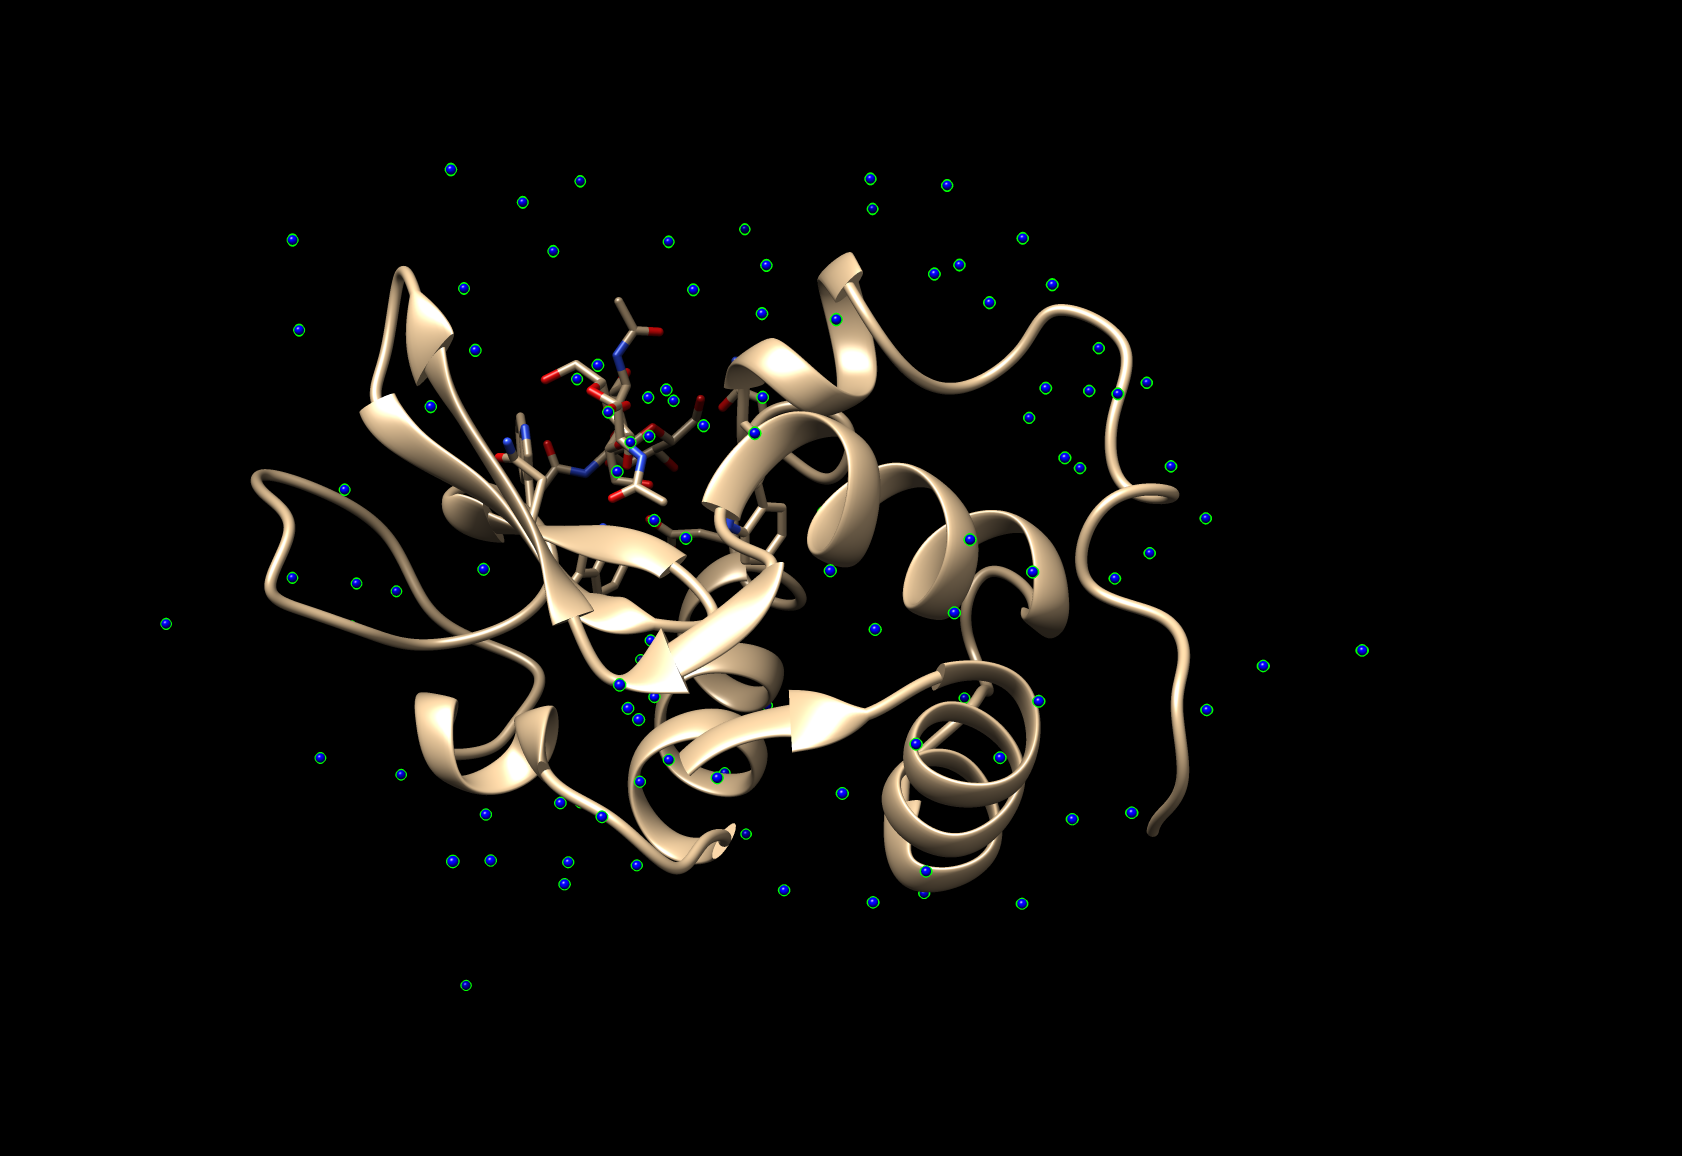
\includegraphics[width=.8\linewidth]{1_c.png}
    \caption{1.c}
    \label{fig:1_c.png}
\end{figure}
\subsection*{(d) Find and mark the ligand. How many atoms does it consist of?}
43 atoms. (and 45 bonds)
\begin{figure}[H]
    \centering
    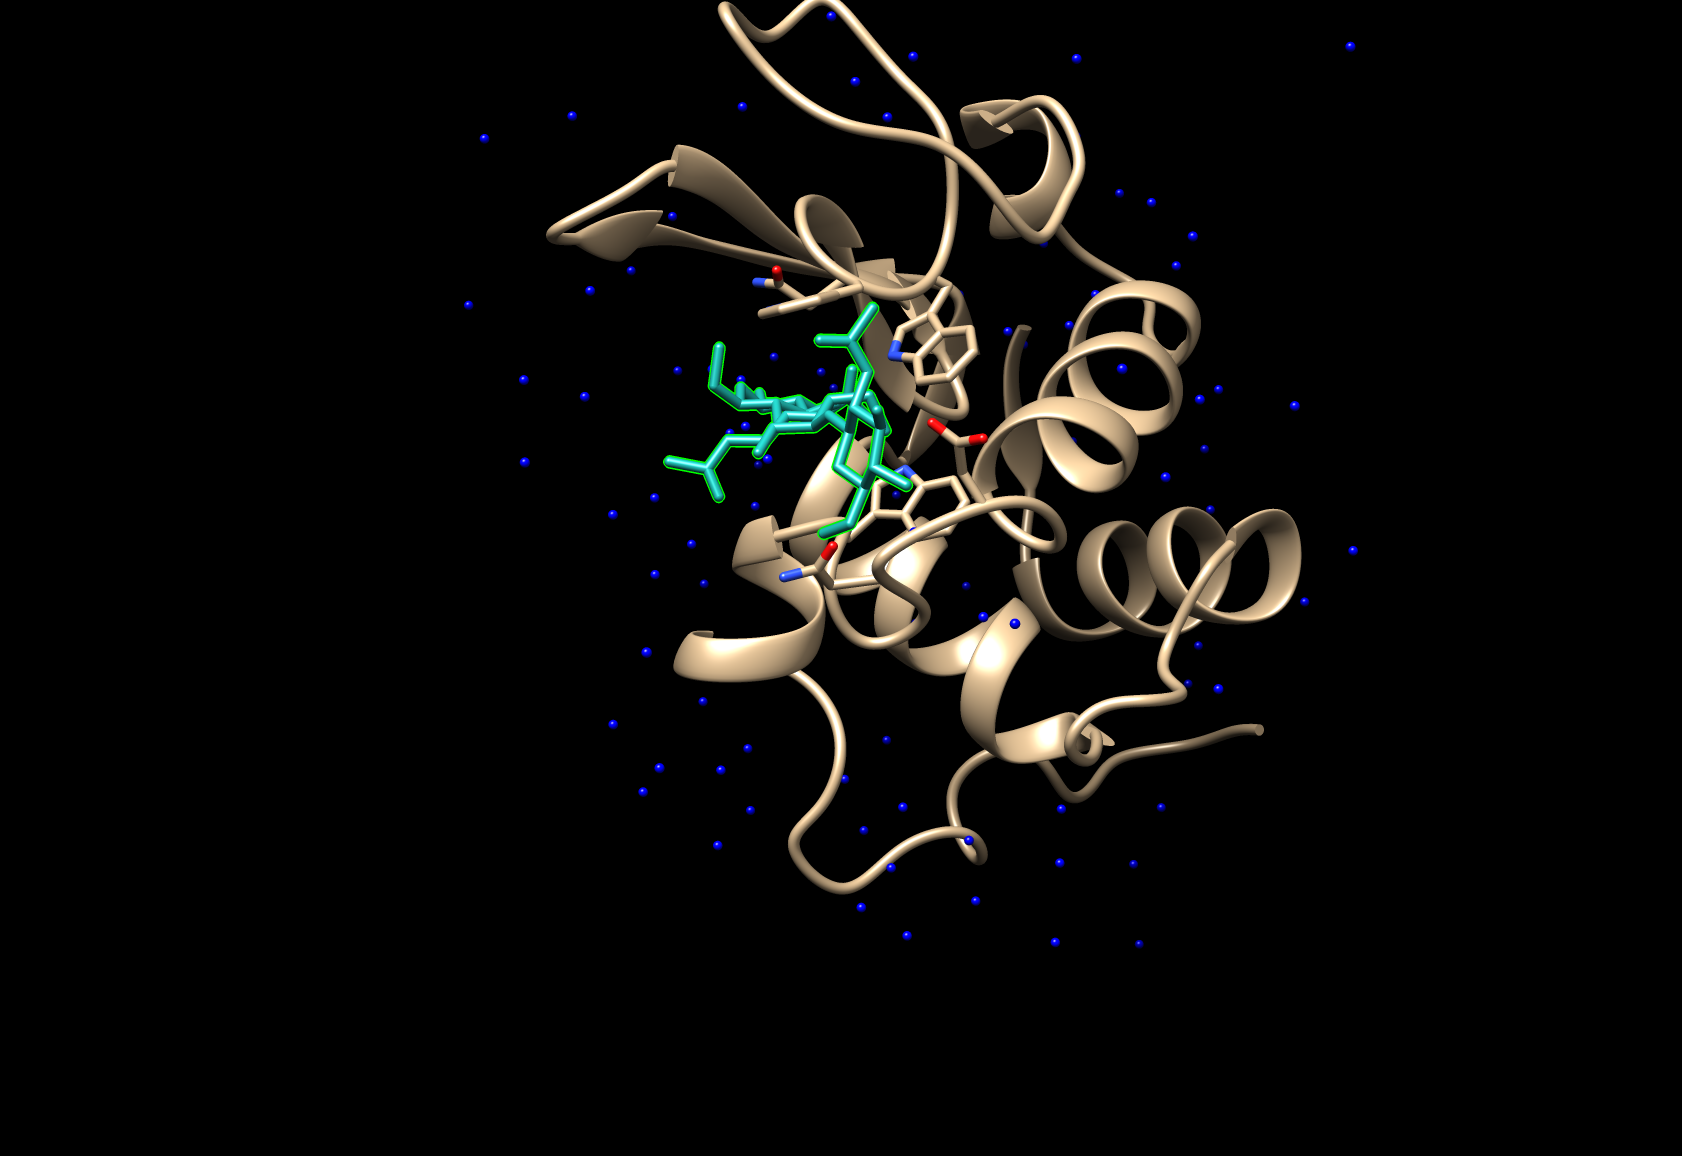
\includegraphics[width=.8\linewidth]{1_d.png}
    \caption{1.d}
    \label{fig:1_d.png}
\end{figure}

\subsection*{(e)Color the protein chain and the ligand in different colors.}
\begin{figure}[H]
    \centering
    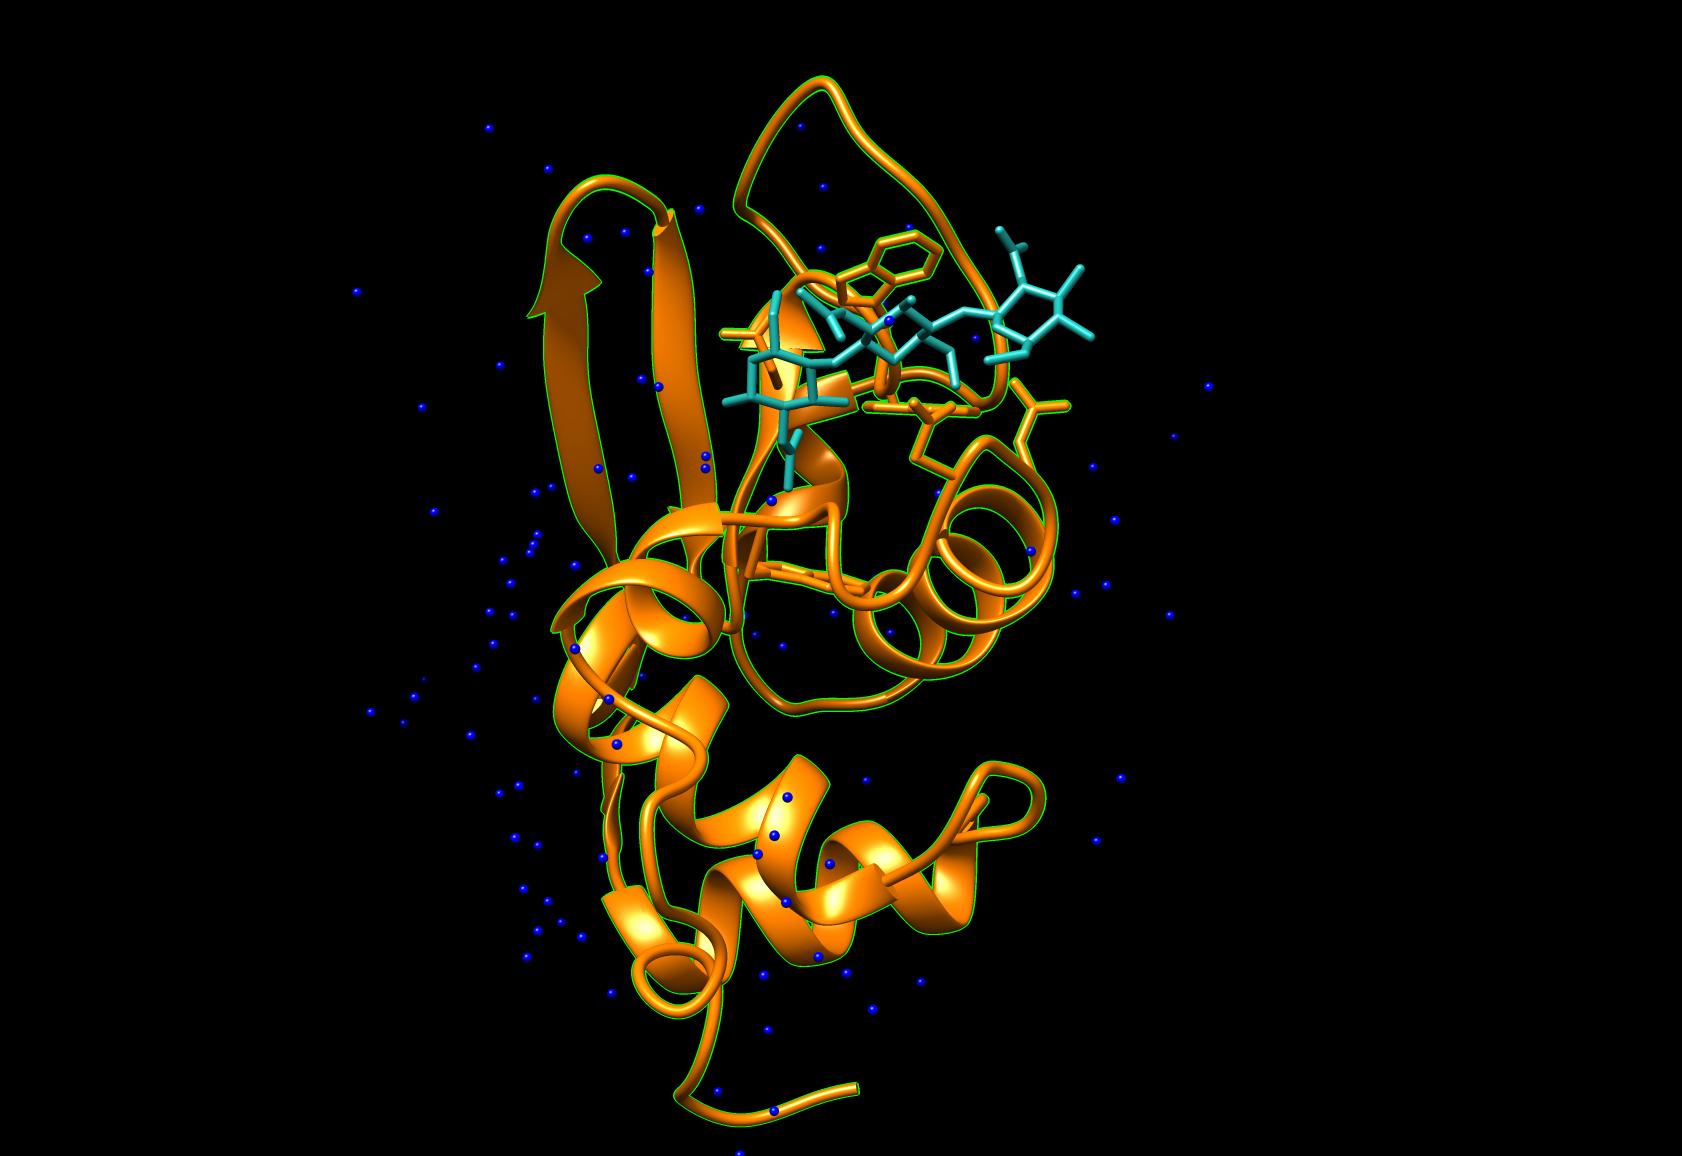
\includegraphics[width=.8\linewidth]{1_e.png}
    \caption{1.e}
    \label{fig:1_e.png}
\end{figure}

\subsection*{(f)Color all the helices the same color.}
\begin{figure}[H]
    \centering
    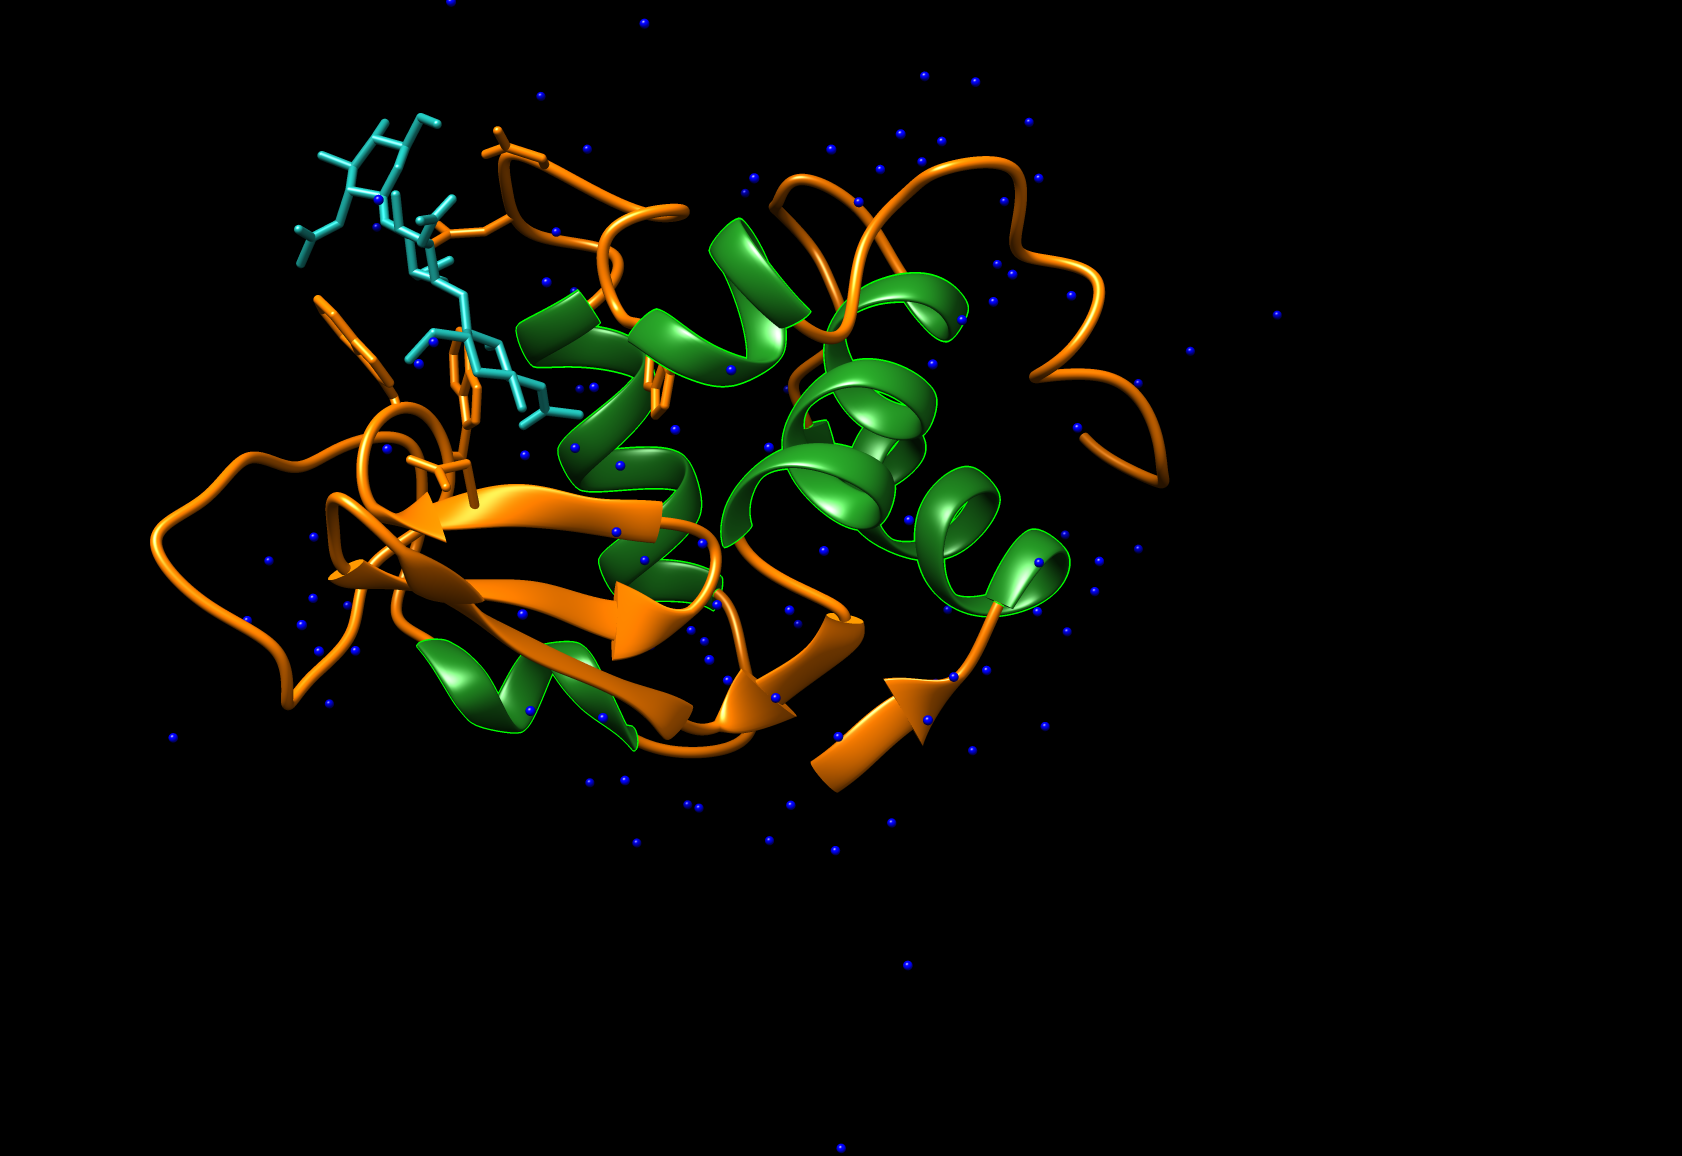
\includegraphics[width=.8\linewidth]{1_f.png}
    \caption{1.f}
    \label{fig:1_f.png}
\end{figure}

\subsection*{(g)Display the surface of the protein chain (only) and set its transparency to 75\%.}
\begin{figure}[H]
    \centering
    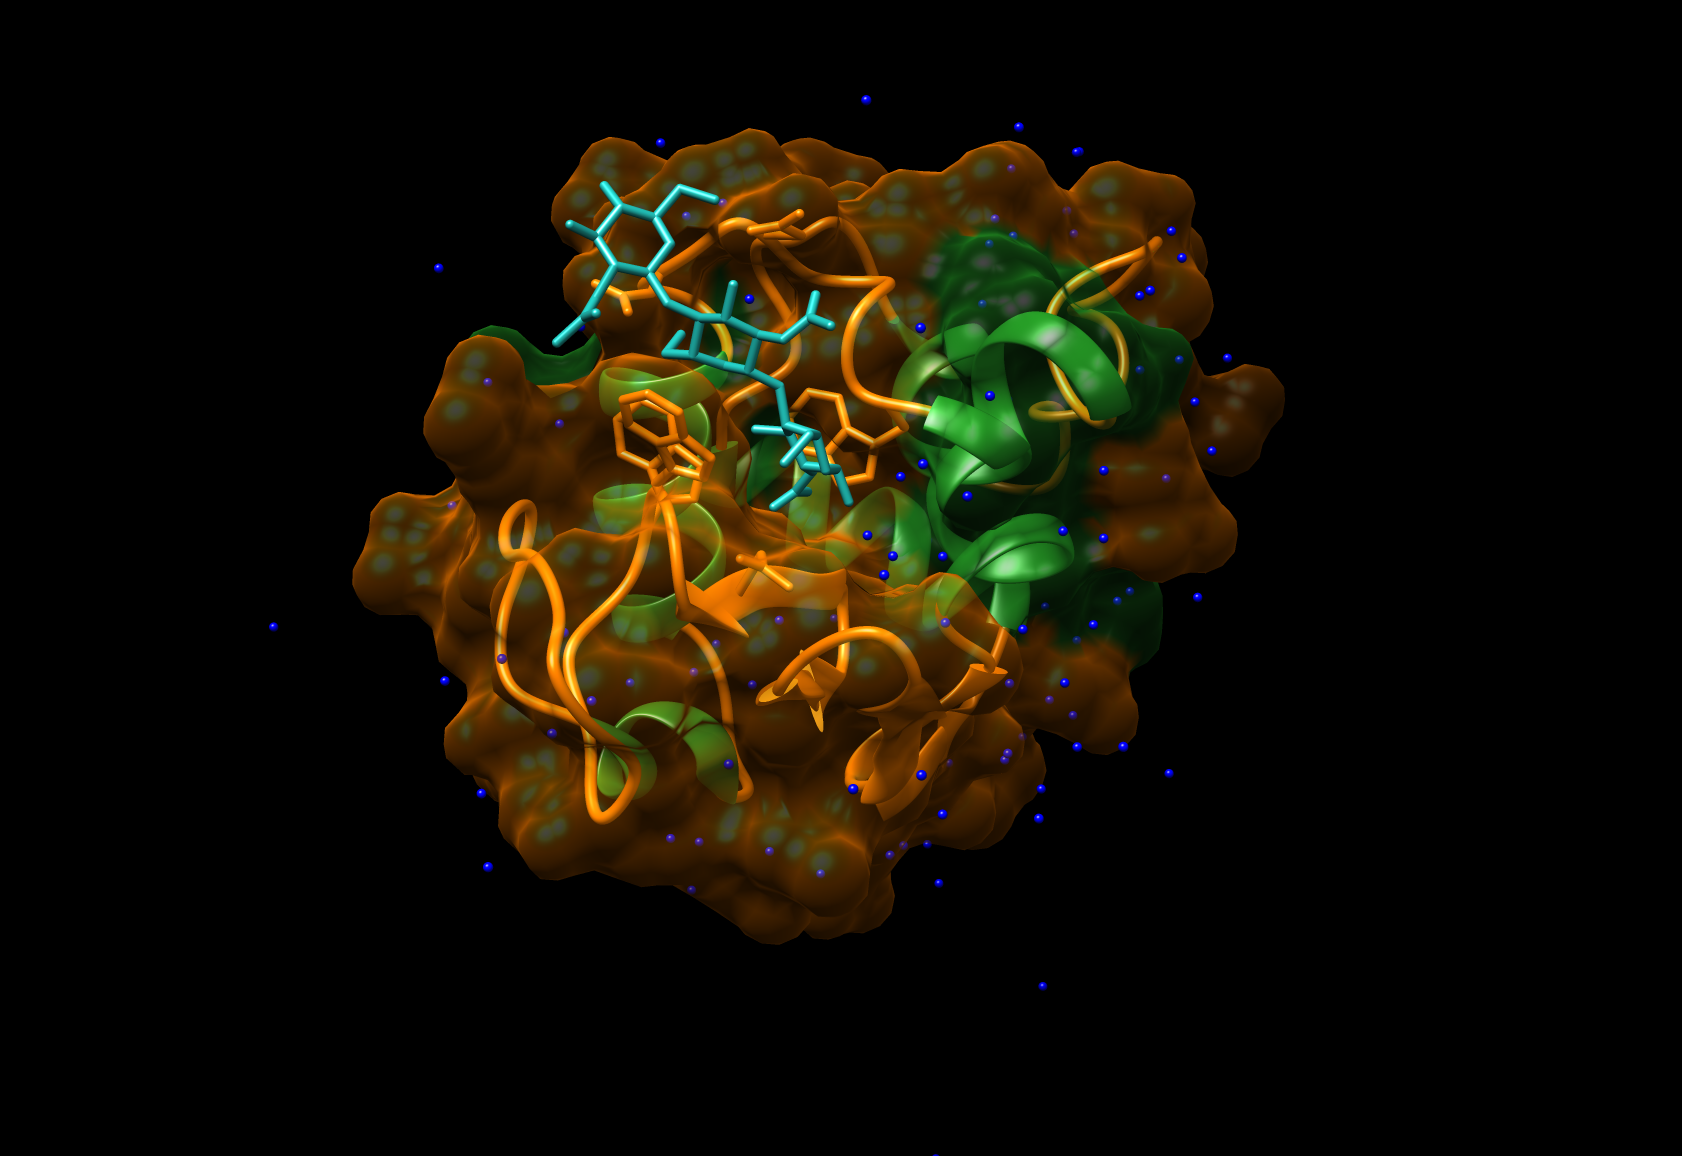
\includegraphics[width=.8\linewidth]{1_g.png}
    \caption{1.g}
    \label{fig:1_g.png}
\end{figure}

\subsection*{(h)Record a video of the rotating structure and attach to the resulting files.}
\subsection*{(i)Save the Chimera sessions (File > Save Session As > .py) and append to the resulting
files as well.}

\section{Exercise 2}
\subsection*{(a)Load the 1BMF structure into Chimera.}
\begin{figure}[H]
    \centering
    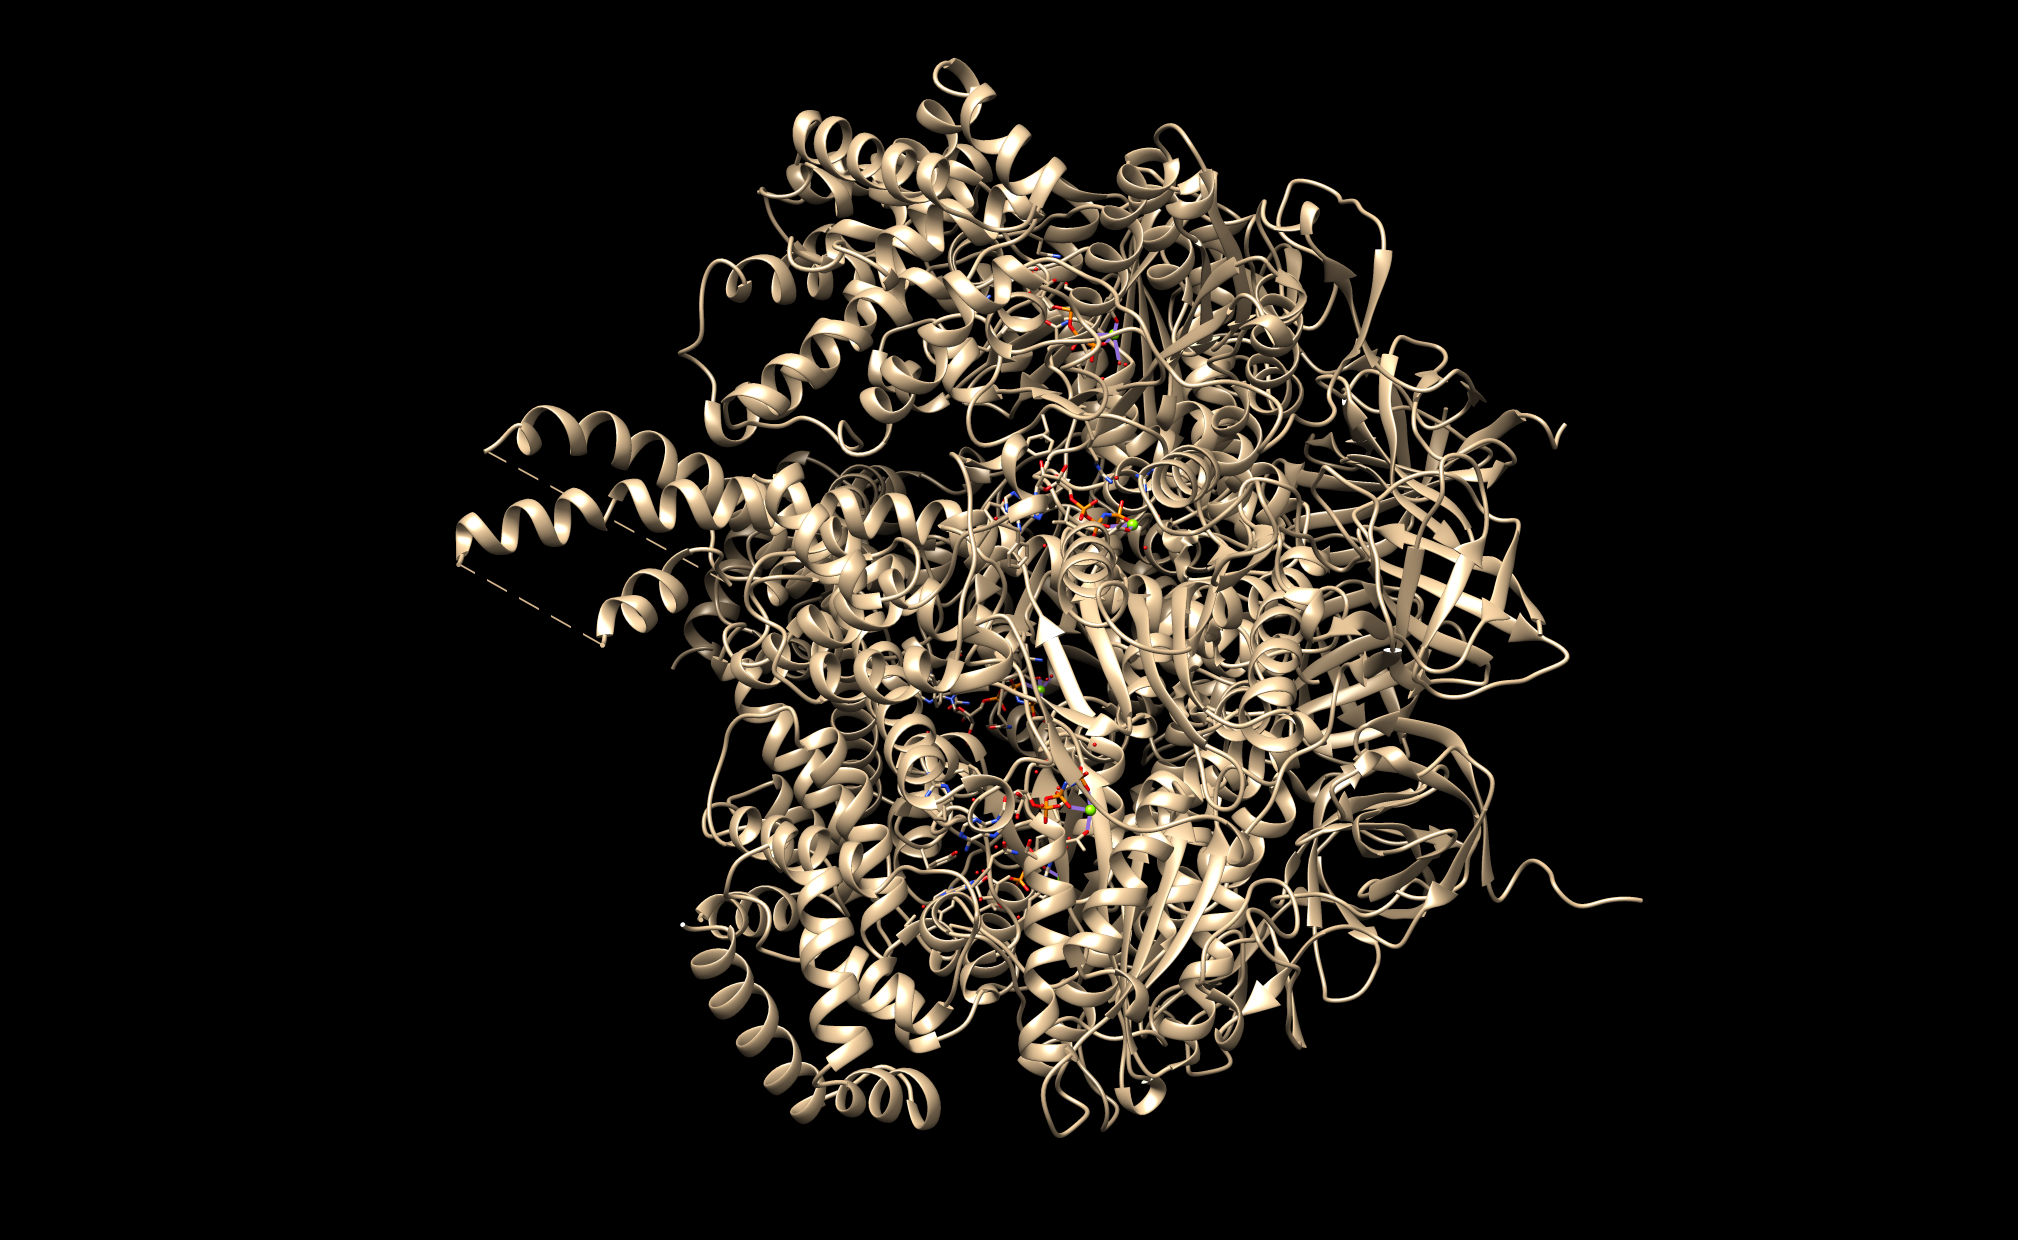
\includegraphics[width=.8\linewidth]{2_a.png}
    \caption{2.a}
    \label{fig:2_a.png}
\end{figure}

\subsection*{(b)What protein are you analyzing?}
BOVINE MITOCHONDRIAL F1-ATPASE\\
PDB DOI: 10.2210/pdb1BMF/pdb\\
Classification: ATP PHOSPHORYLASE\\
Organism(s): Bos taurus\\
Mutation(s): Yes \\
Membrane Protein: Yes  mpstruc\\

Deposited: 1996-03-13 Released: 1996-12-07 \\
Deposition Author(s): Abrahams, J.P., Leslie, A.G.W., Lutter, R., Walker, J.E.\\
Experimental Data Snapshot\\

Method: X-RAY DIFFRACTION\\
Resolution: 2.85 Å\\

\subsection*{(c)How many chains does this protein have? Color each of them a different color with
Rainbow.}
7 chains.\\
\begin{figure}[H]
    \centering
    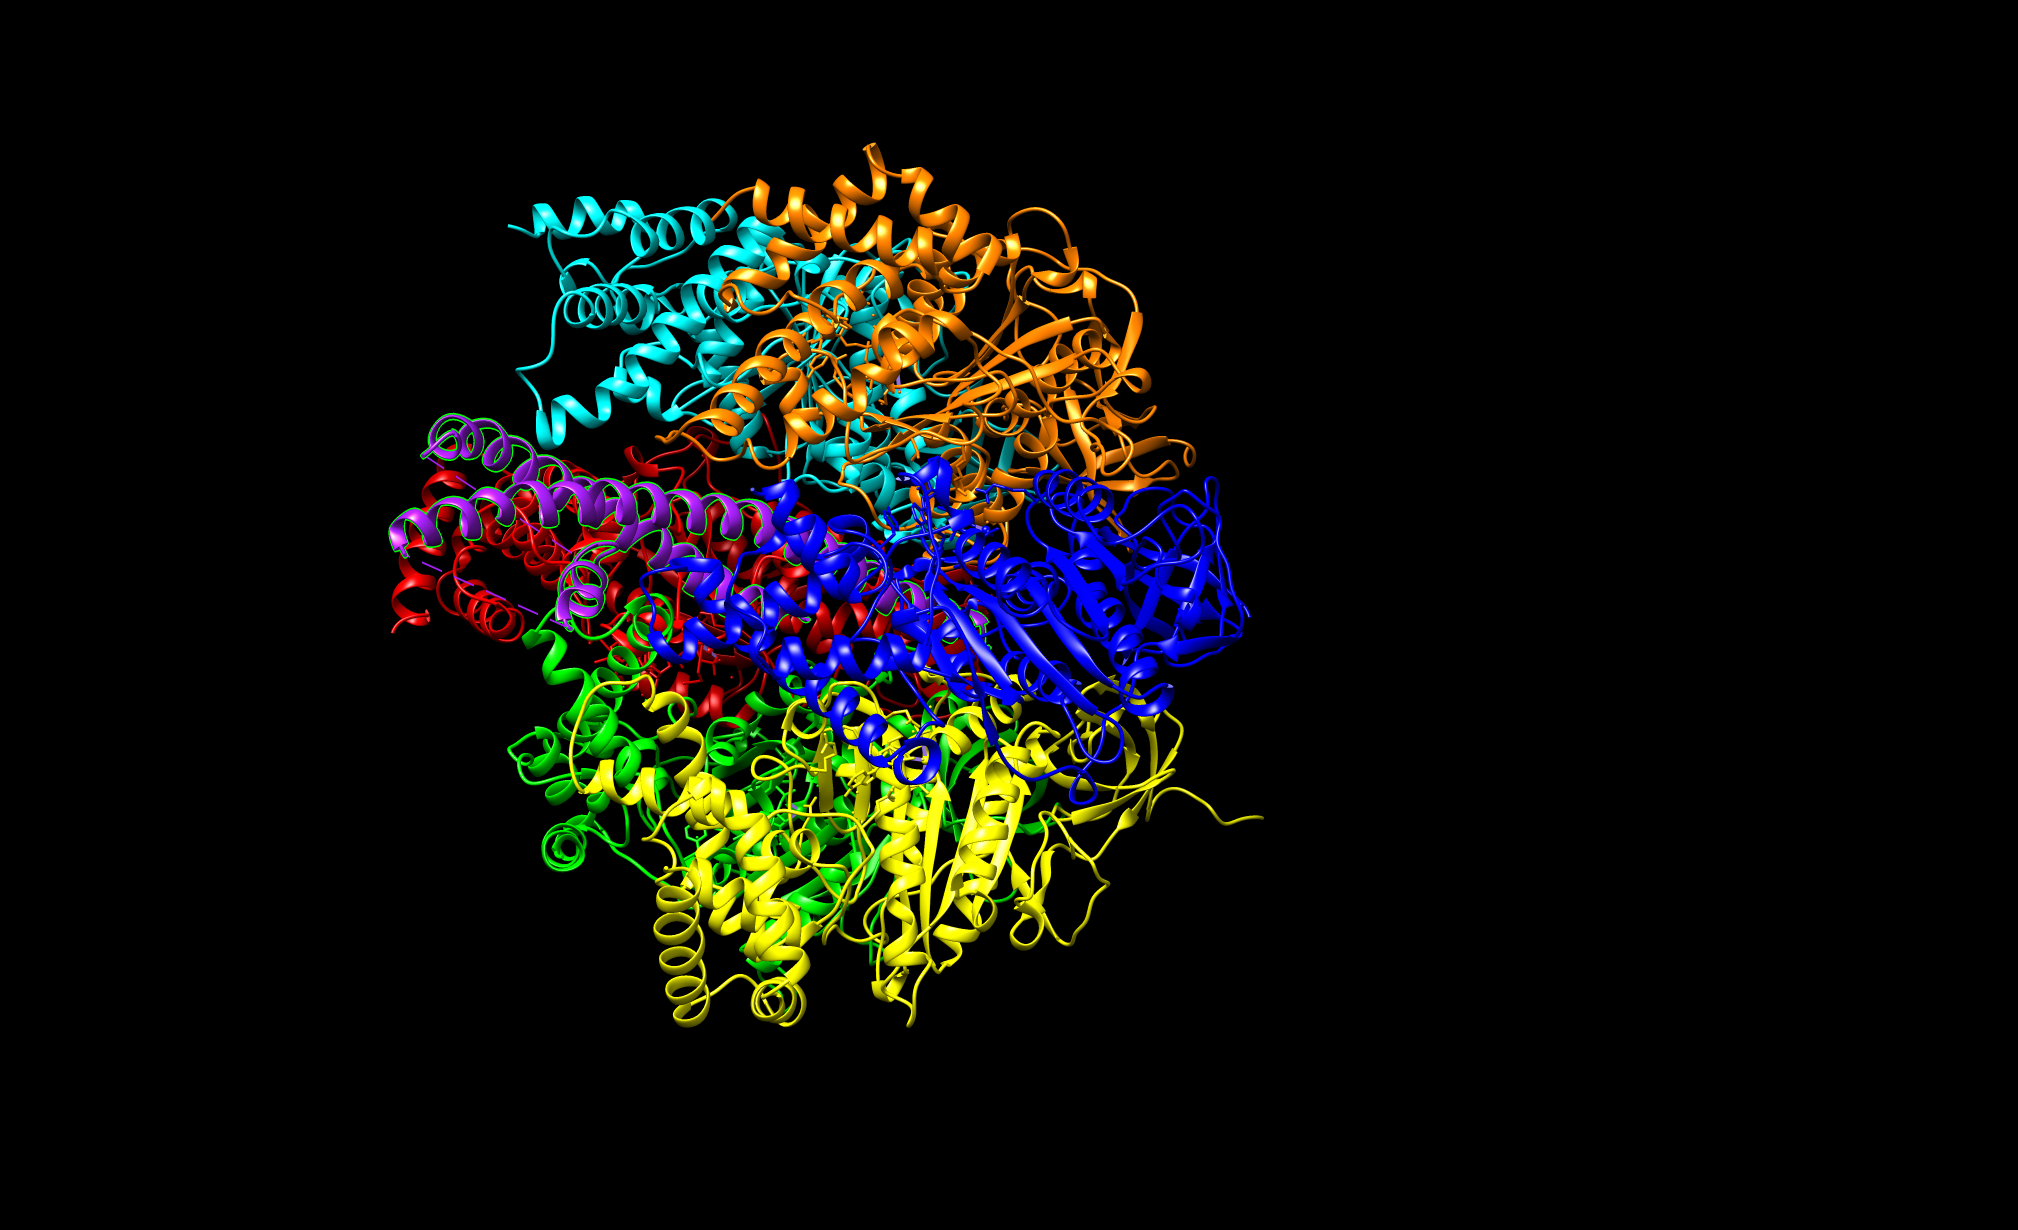
\includegraphics[width=.8\linewidth]{2_c.png}
    \caption{2.c}
    \label{fig:2_c.png}
\end{figure}

\subsection*{(d) How many ligands are in this protein? Display the surface of each of them.}
5 ligands.\\
\begin{figure}[H]
    \centering
    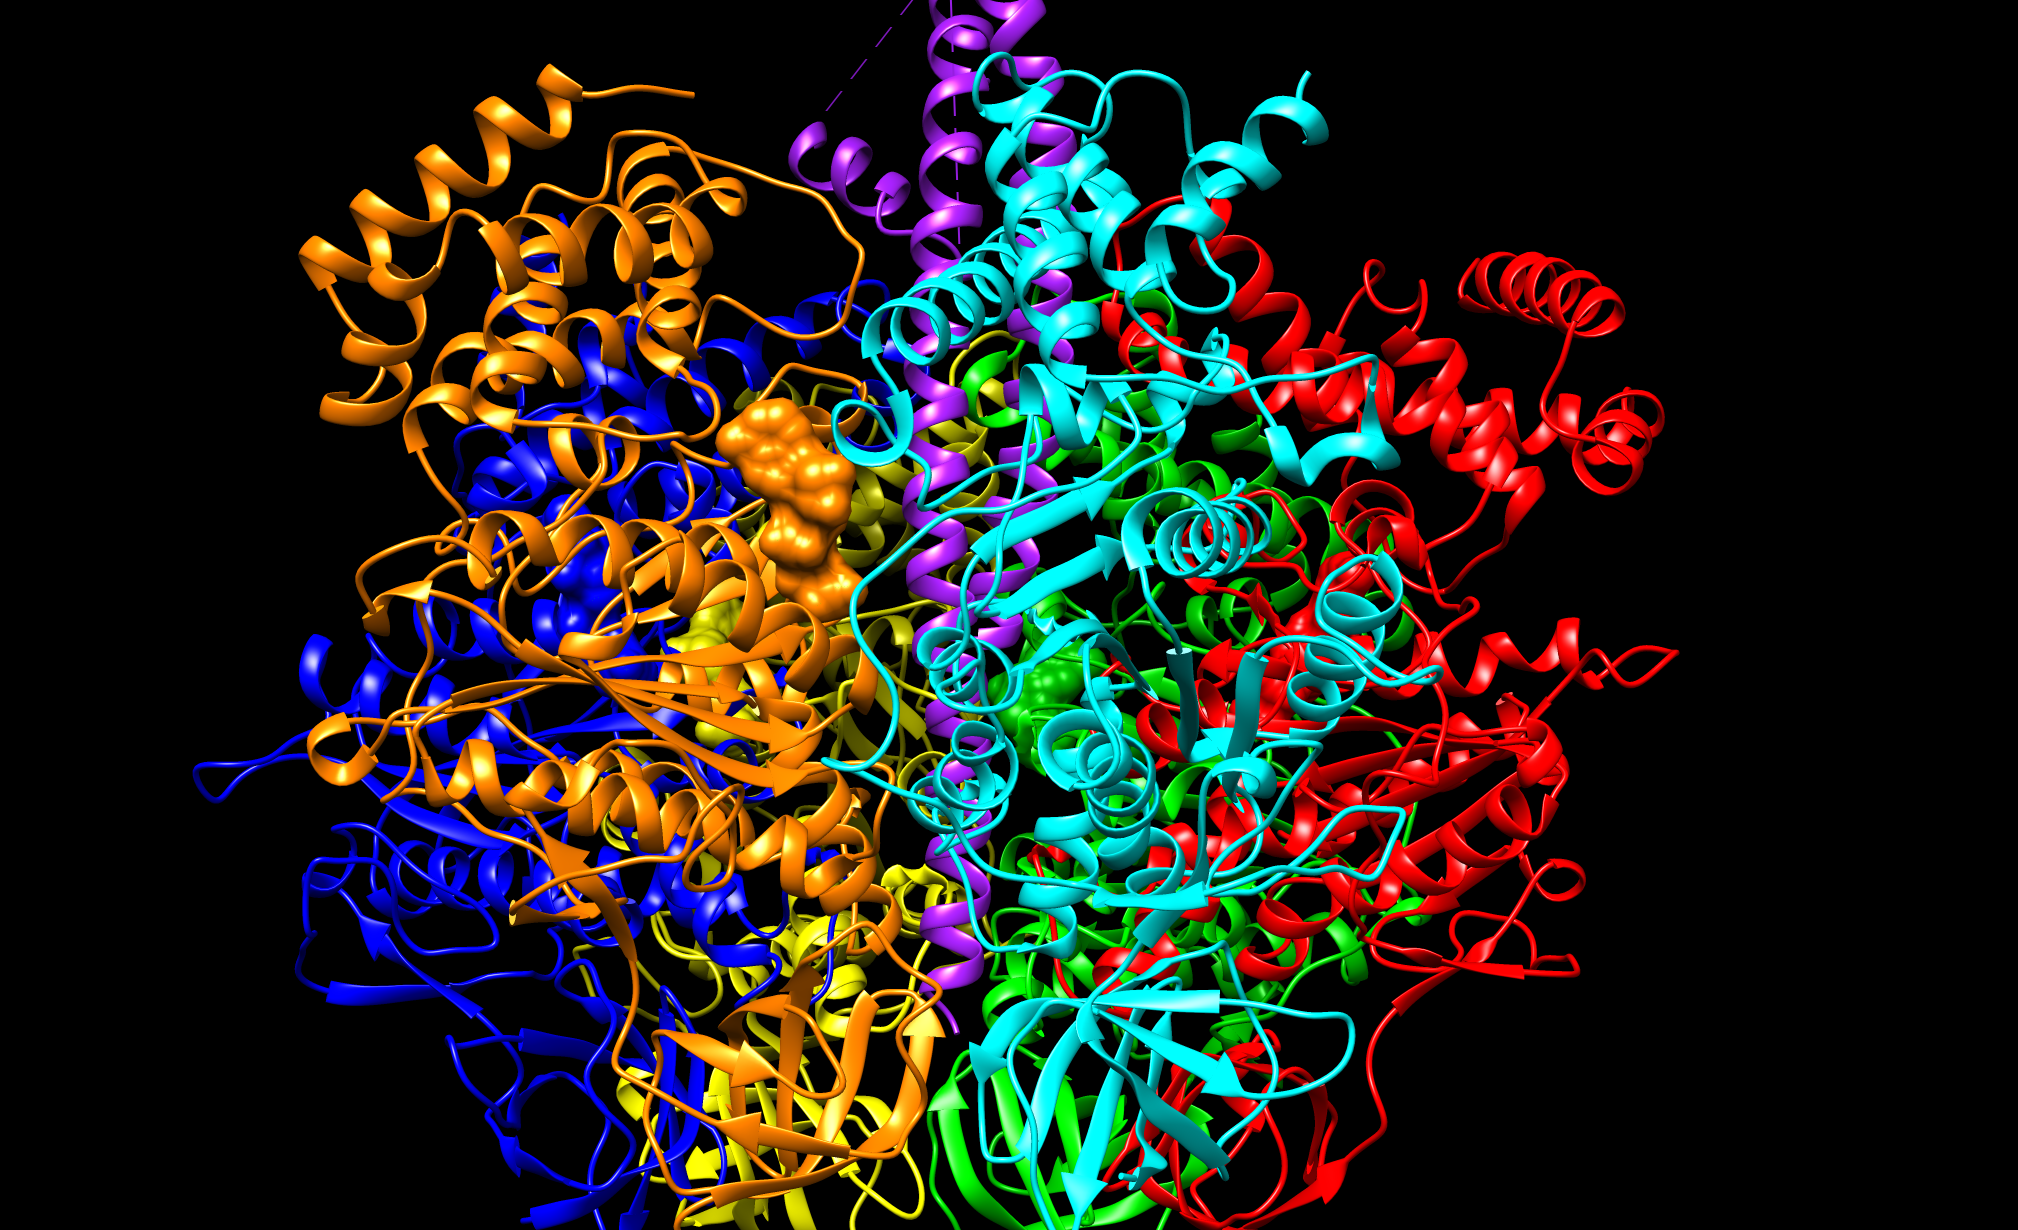
\includegraphics[width=.8\linewidth]{2_d.png}
    \caption{2.d}
    \label{fig:2_d.png}
\end{figure}
\begin{figure}[H]
    \centering
    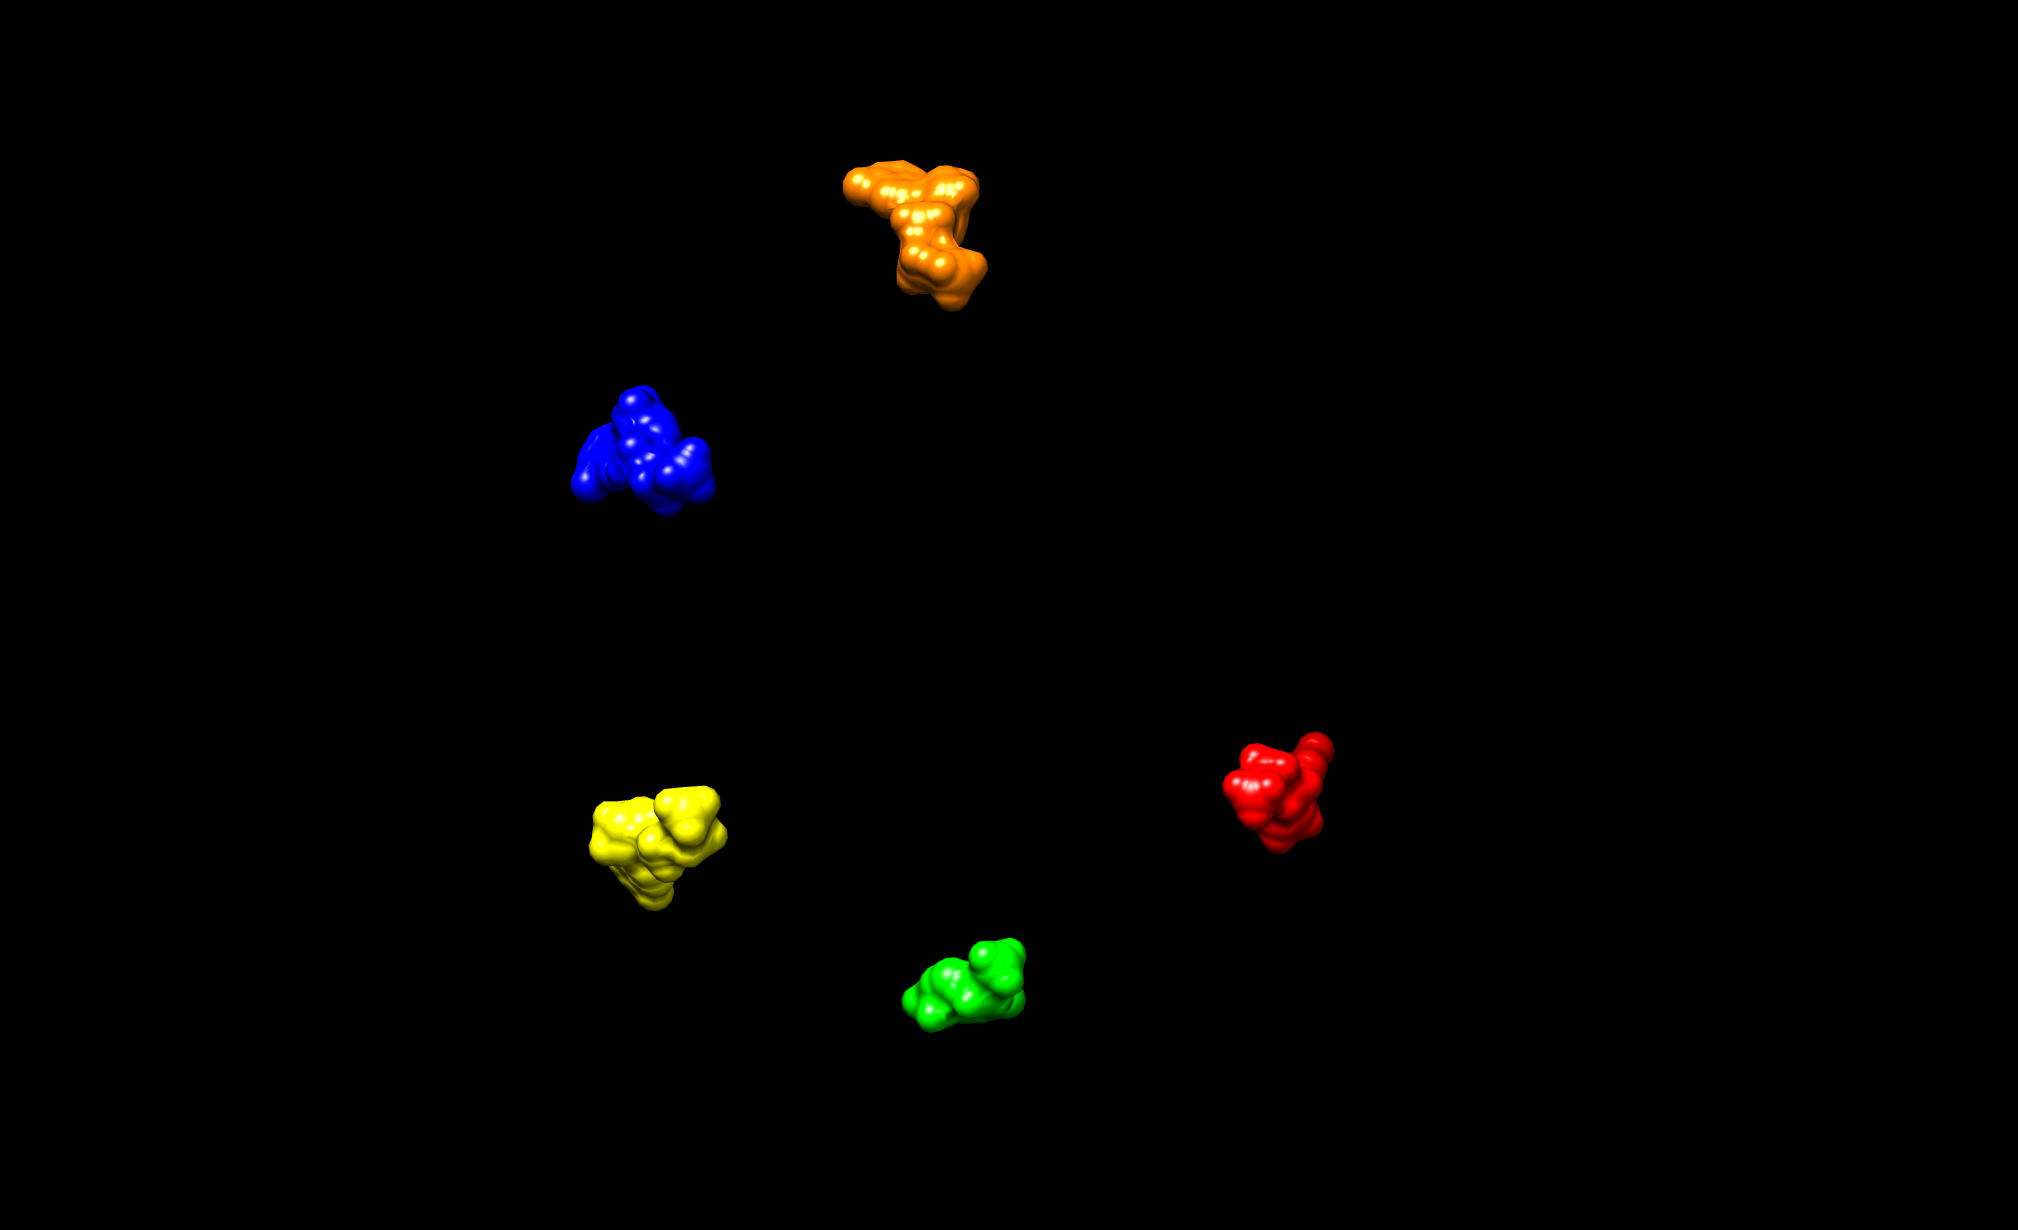
\includegraphics[width=.8\linewidth]{2_d2.png}
    \caption{2.d2}
    \label{fig:2_d2.png}
\end{figure}
\subsection*{(e) Display all hydrogen bonds in a protein.}
\begin{figure}[H]
    \centering
    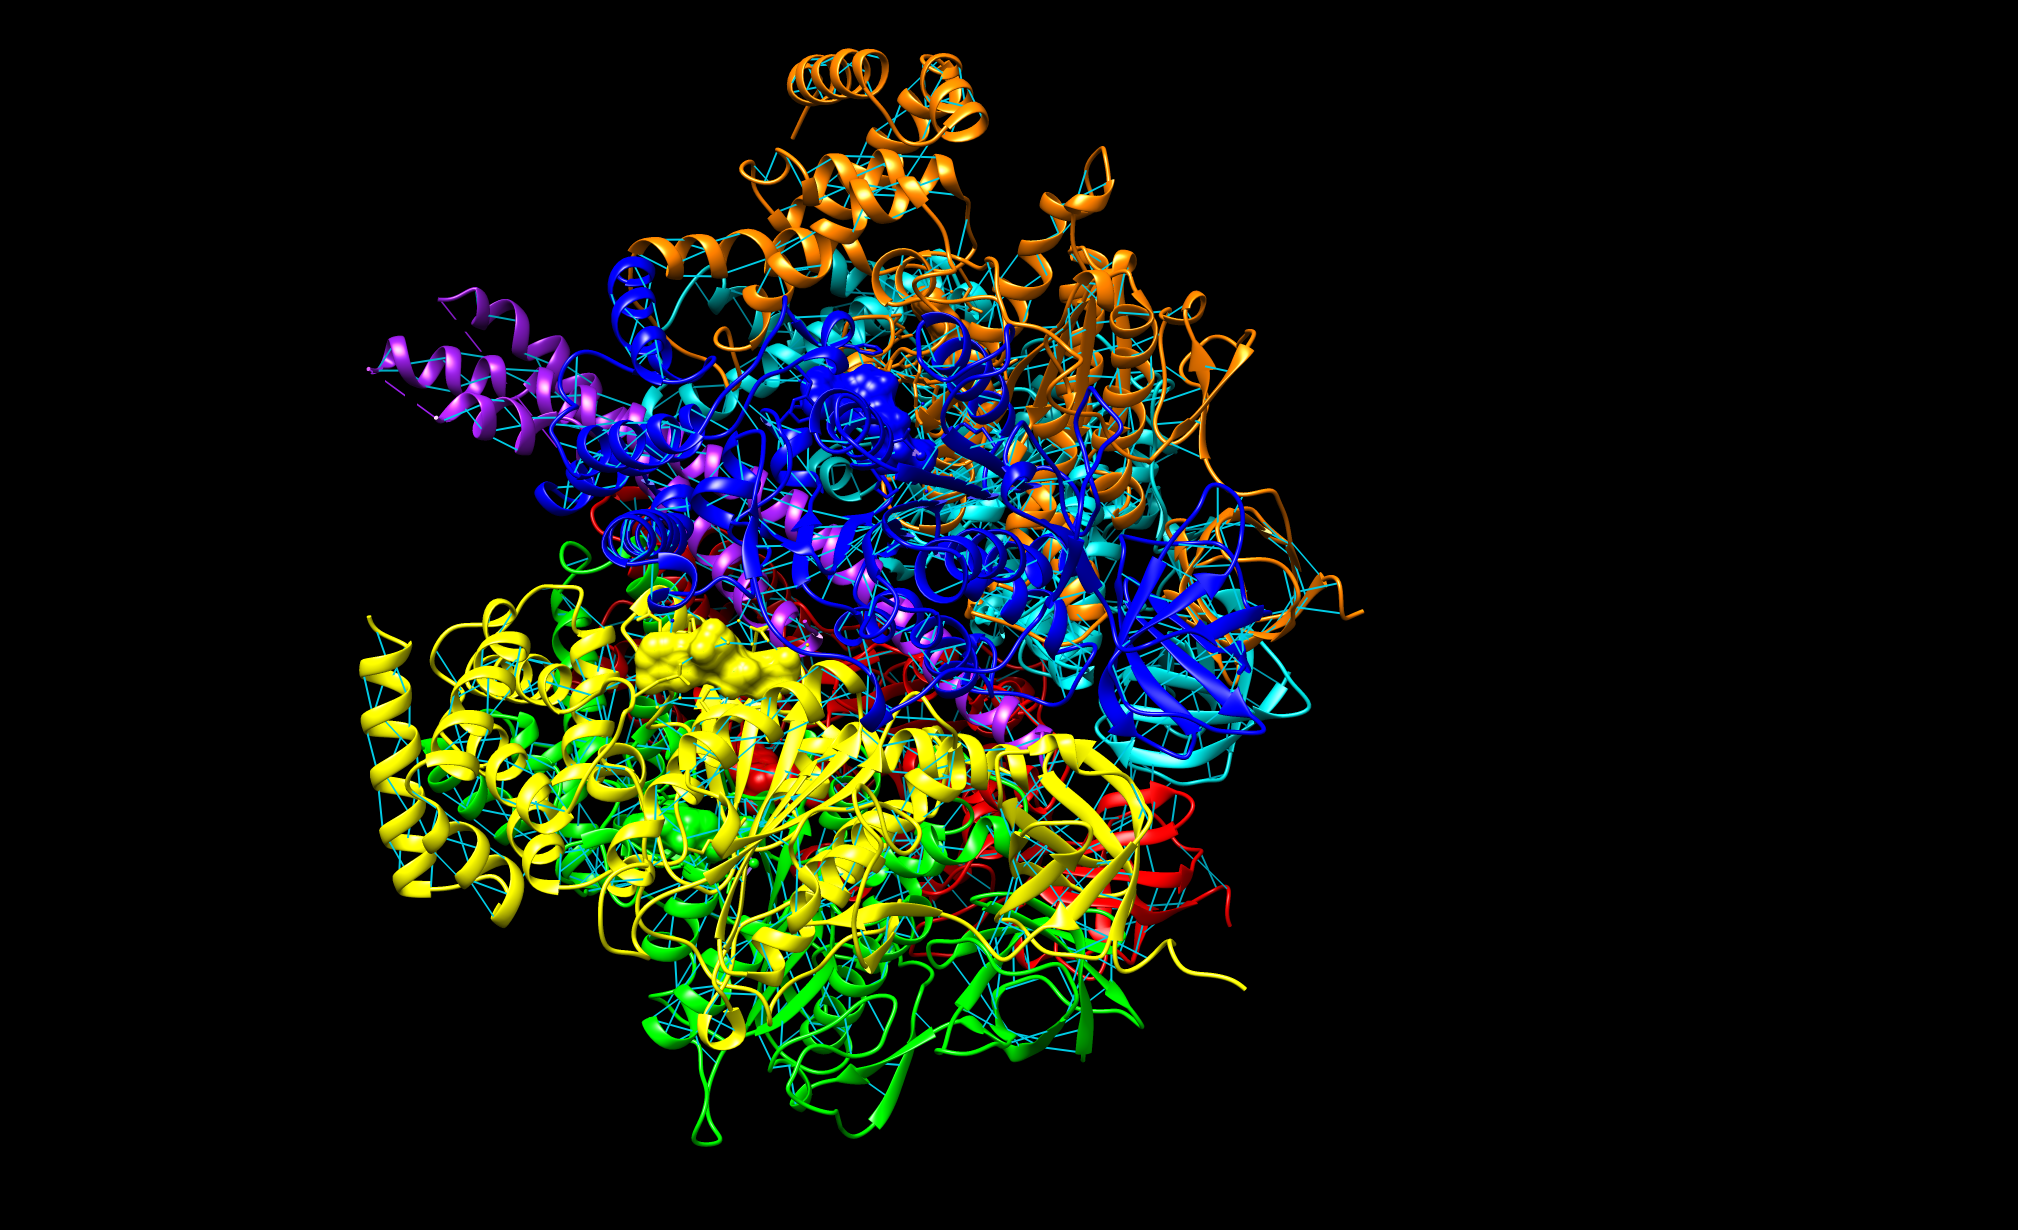
\includegraphics[width=.8\linewidth]{2_e.png}
    \caption{2.e}
    \label{fig:2_e.png}
\end{figure}
\subsection*{(f) Display the surface of all chains. Which hydrogen bonds cross it?}
There are HOH molecules outside the surface.\\
The hydrogen bonds could cross the surface if one end of the bond is a HOH molecule outside the surface and the other end inside the surface. 
\begin{figure}[H]
    \centering
    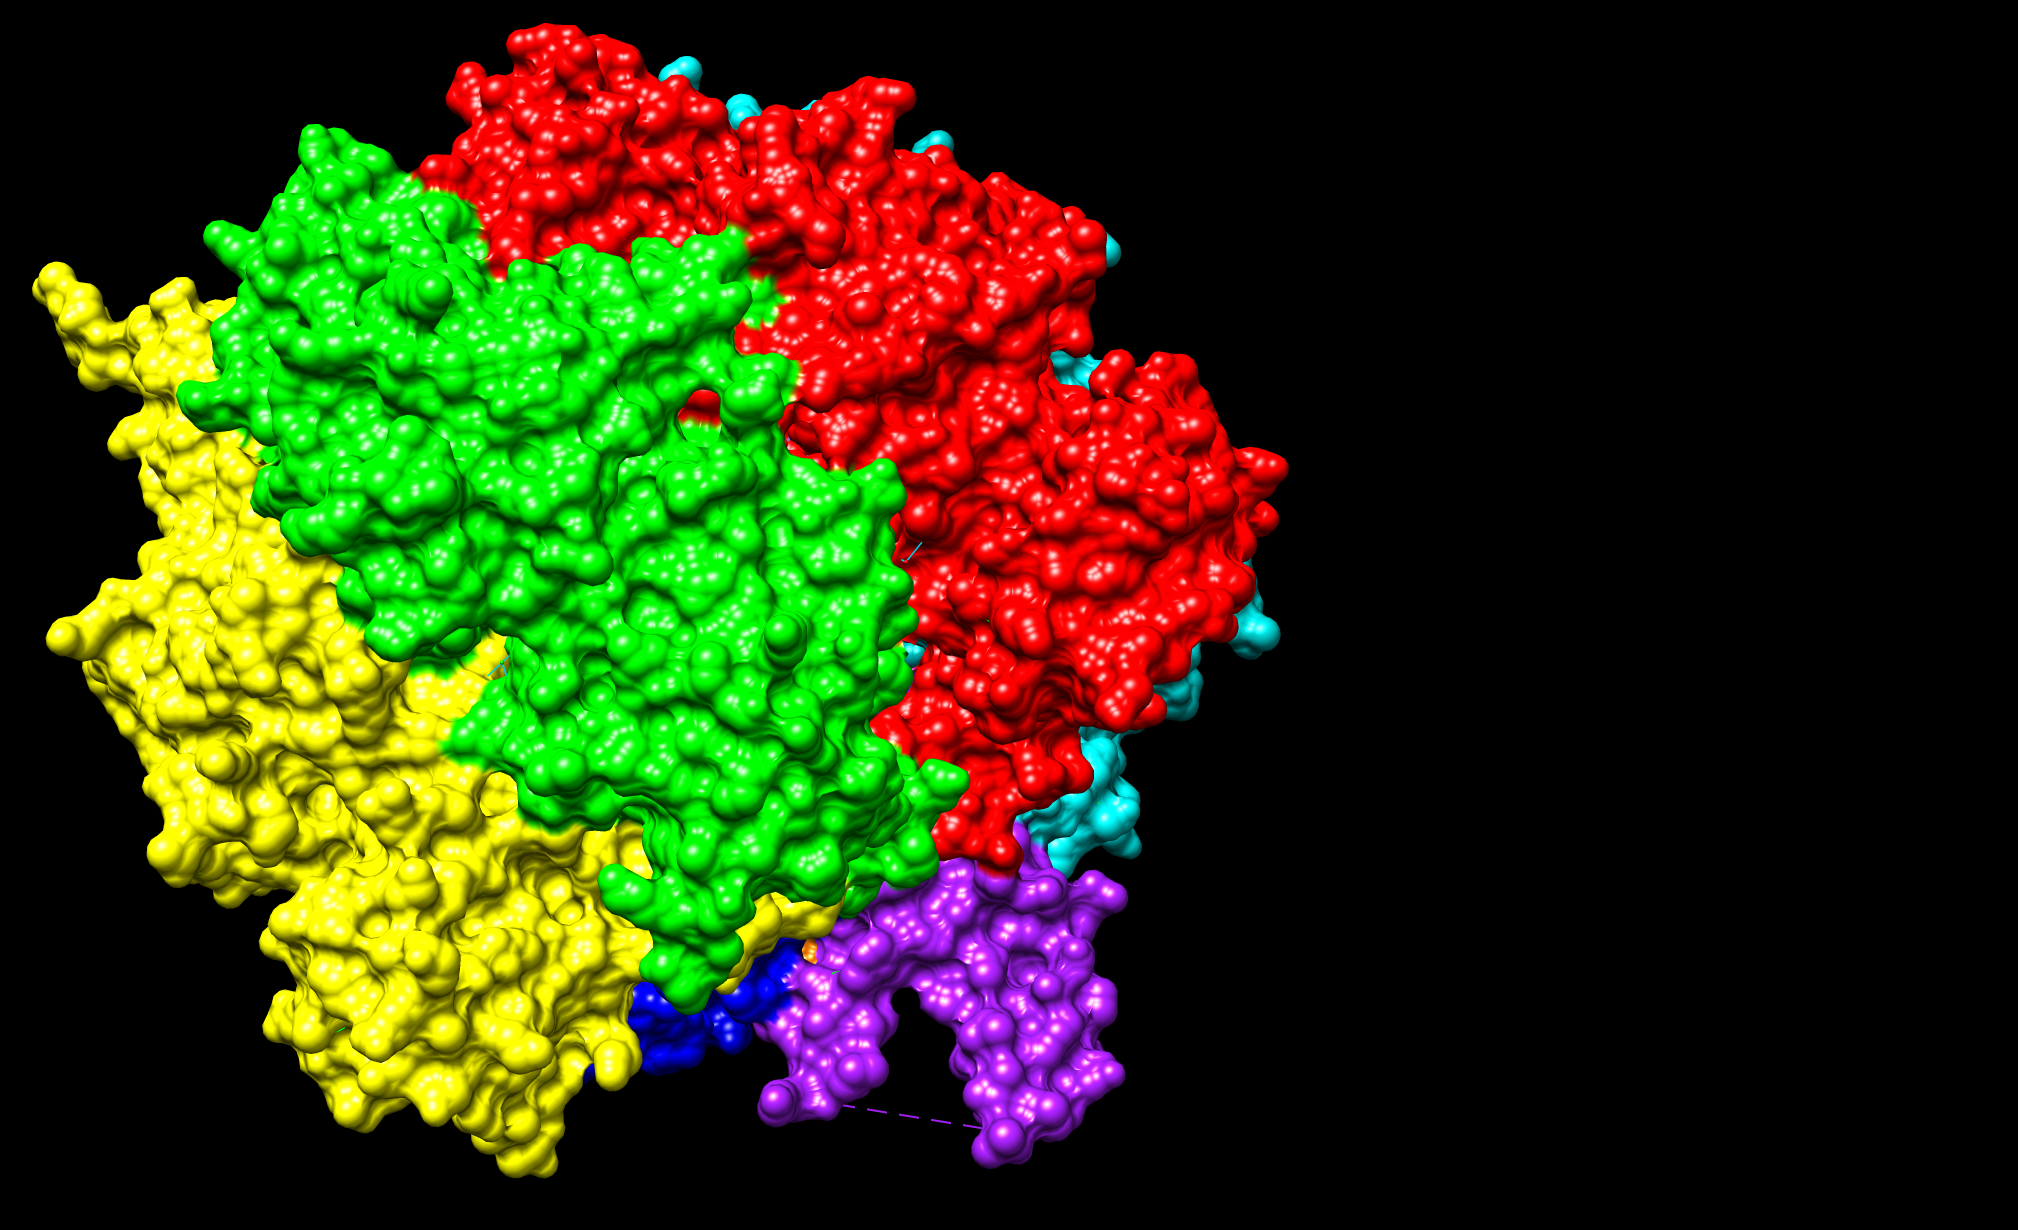
\includegraphics[width=.8\linewidth]{2_f.png}
    \caption{2.f}
    \label{fig:2_f.png}
\end{figure}
\subsection*{(g) Remove the chain that is in the middle of the protein.}
\begin{figure}[H]
    \centering
    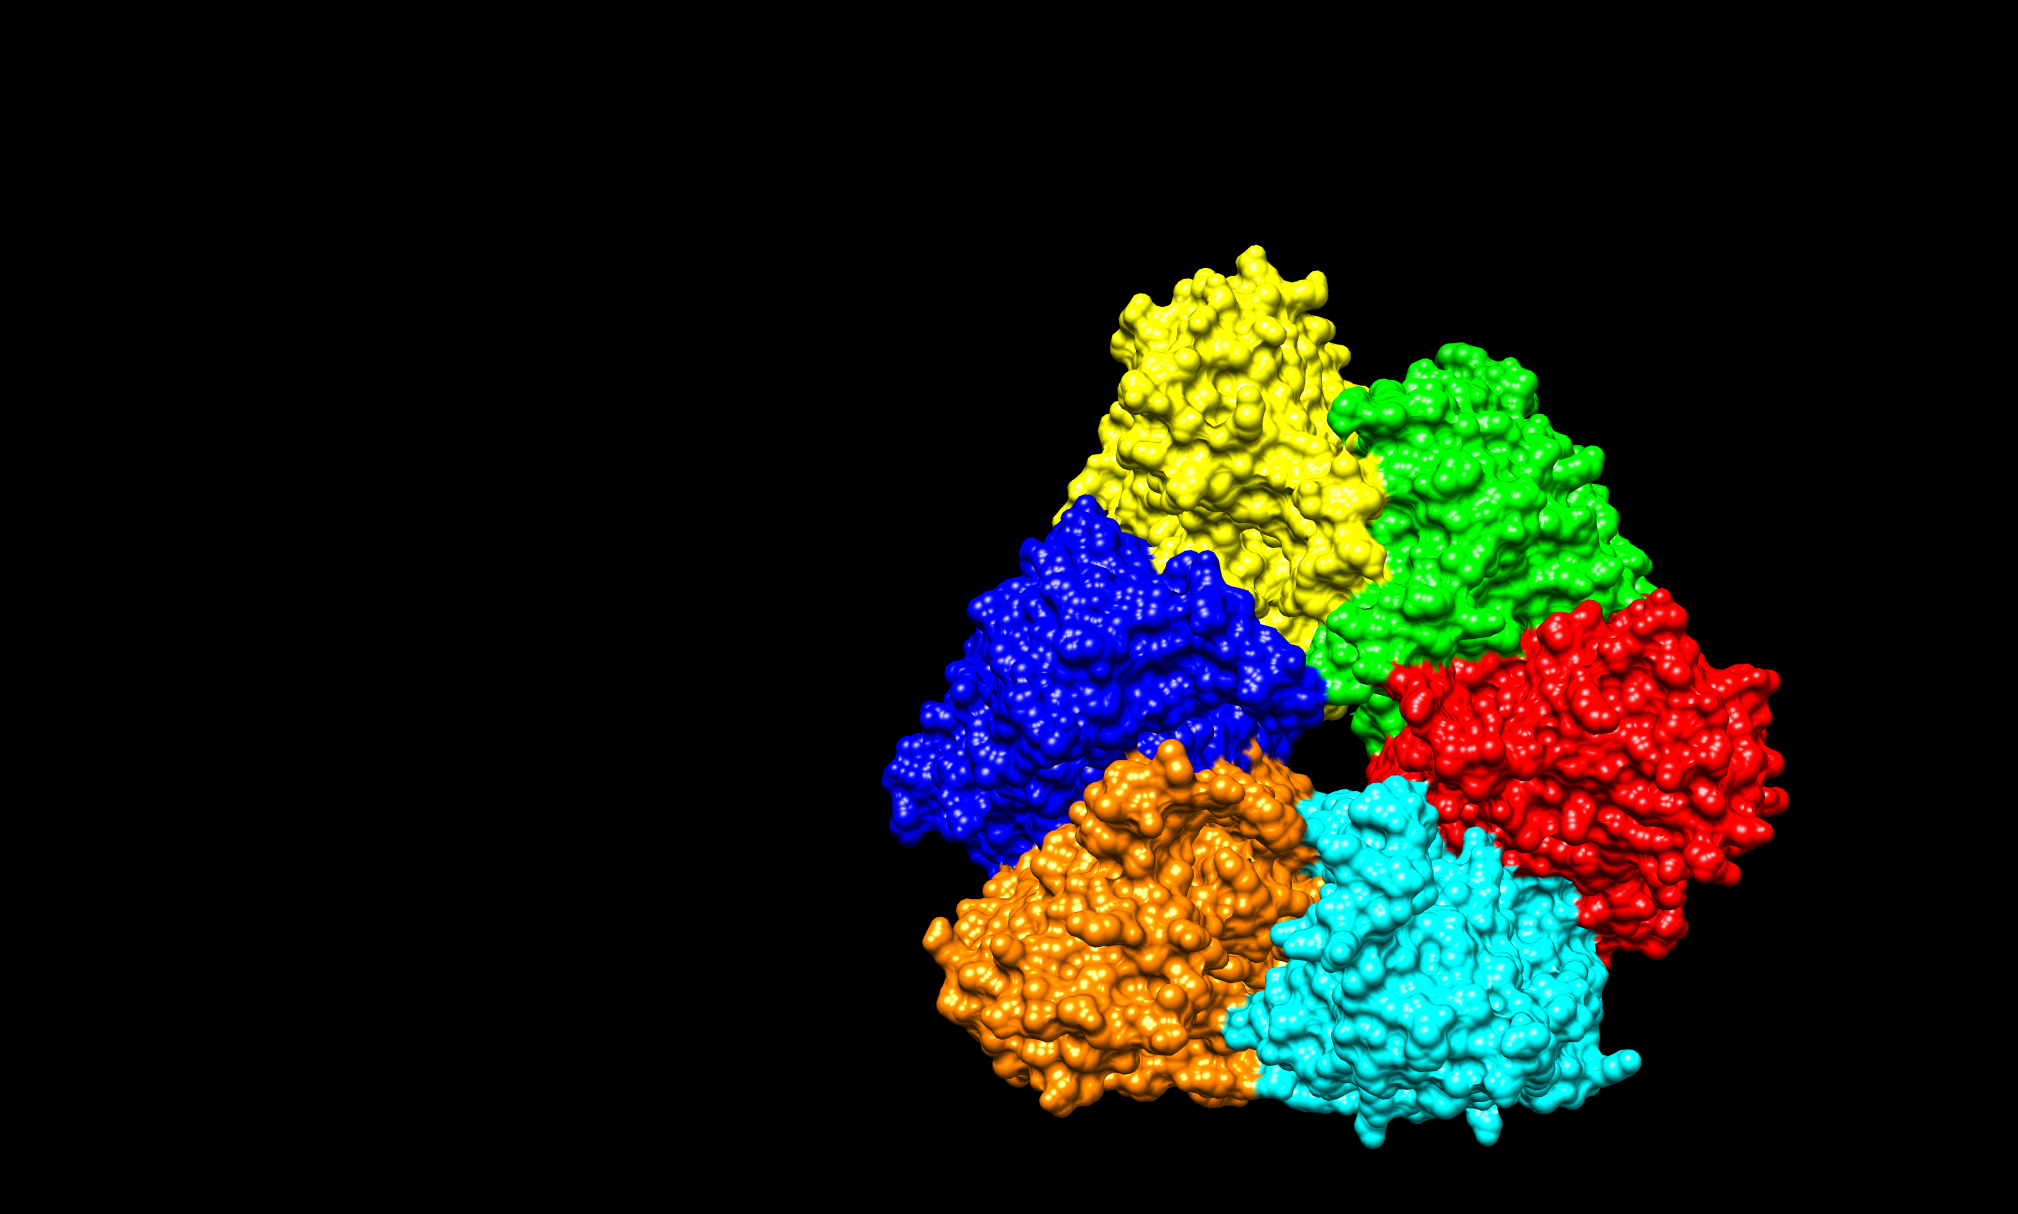
\includegraphics[width=.8\linewidth]{2_g.png}
    \caption{2.g}
    \label{fig:2_g.png}
\end{figure}
\subsection*{(h) Remove all water particles. Has there been any change in hydrogen bonding?}
There are no more hydrogen bonding cross the surface, because the HOH molecules are removed.
\begin{figure}[H]
    \centering
    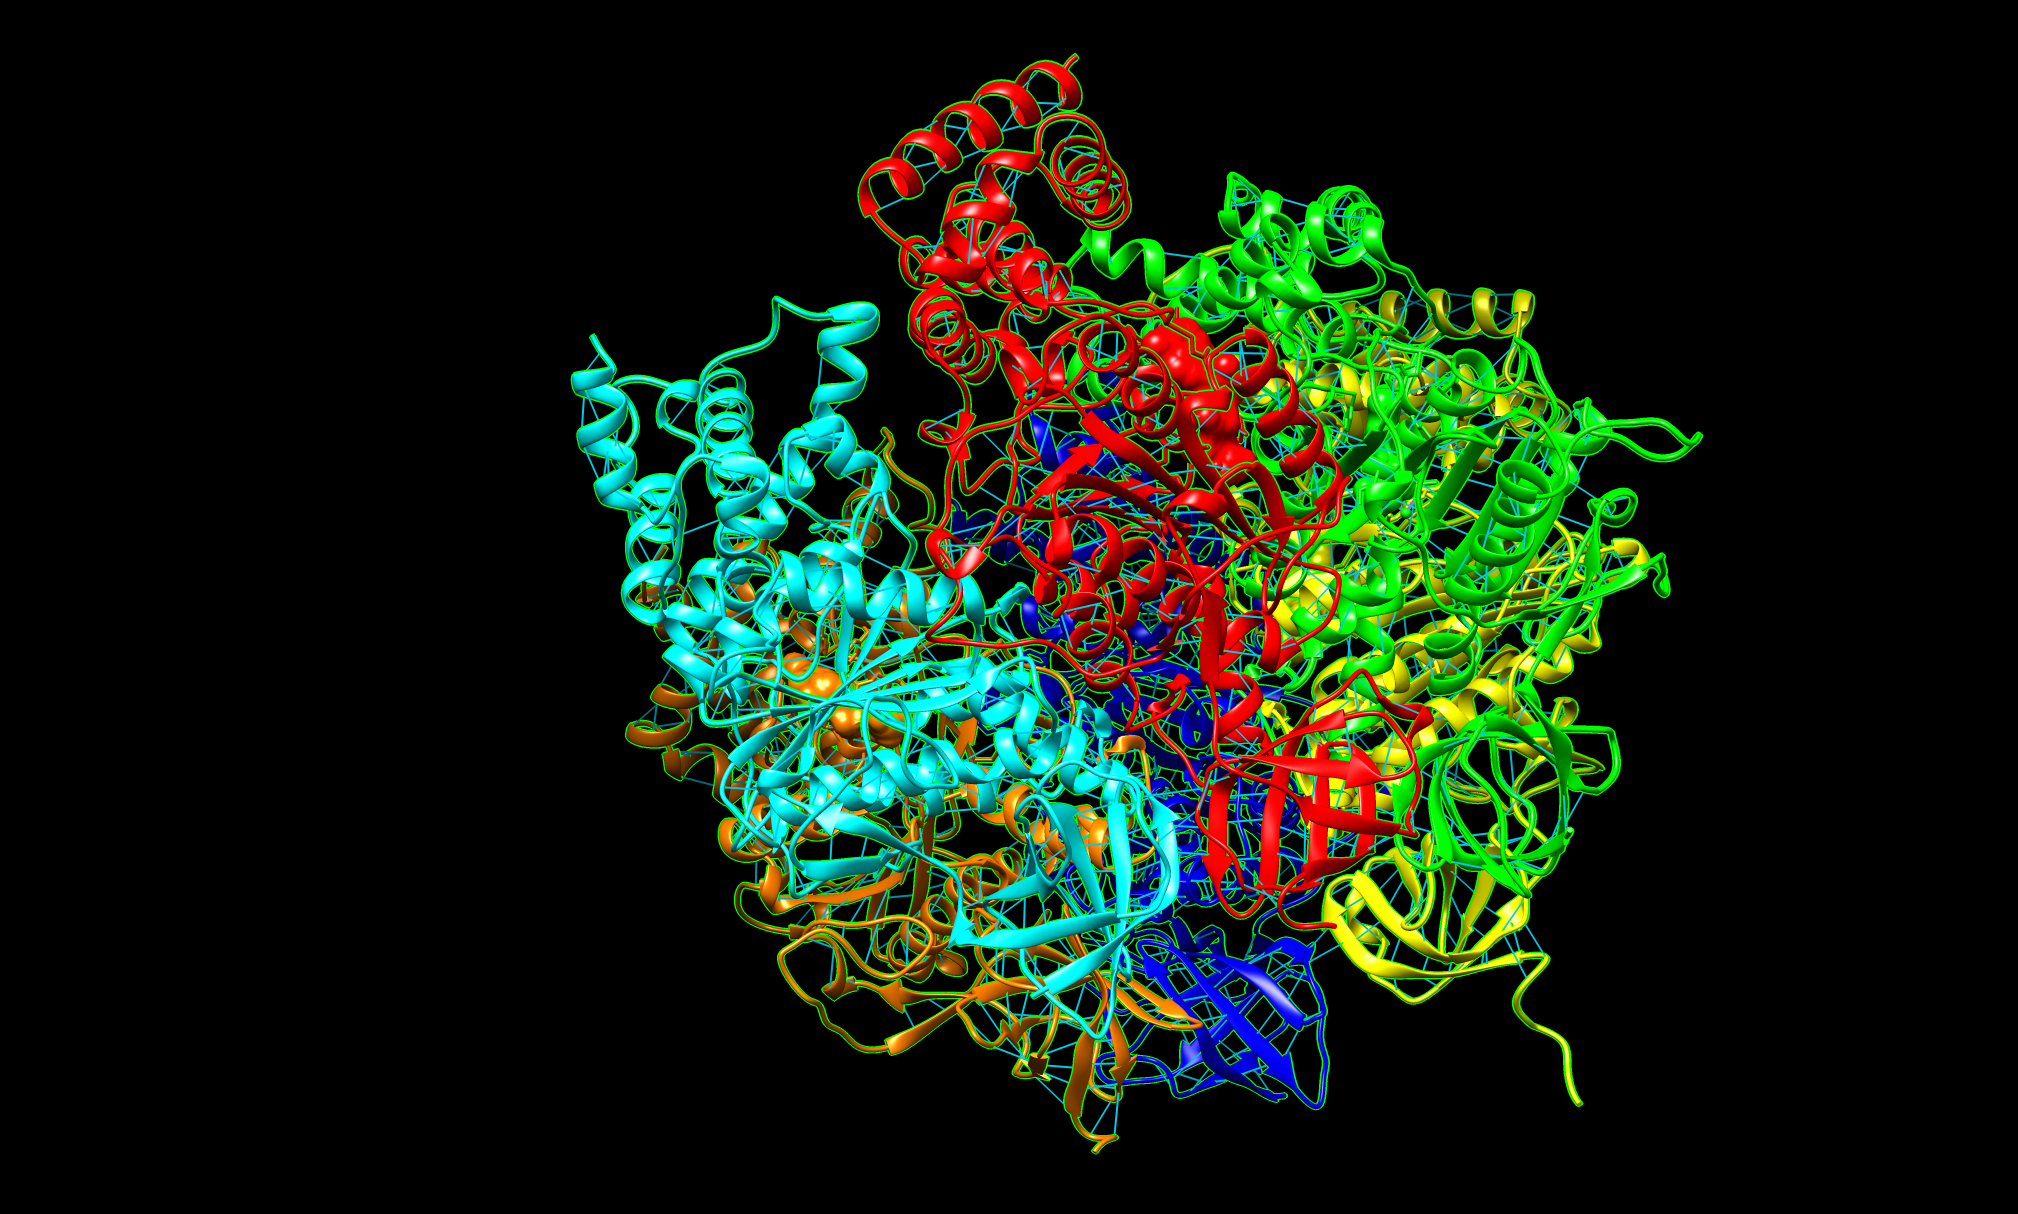
\includegraphics[width=.8\linewidth]{2_h.png}
    \caption{2.h}
    \label{fig:2_h.png}
\end{figure}
\begin{figure}[H]
    \centering
    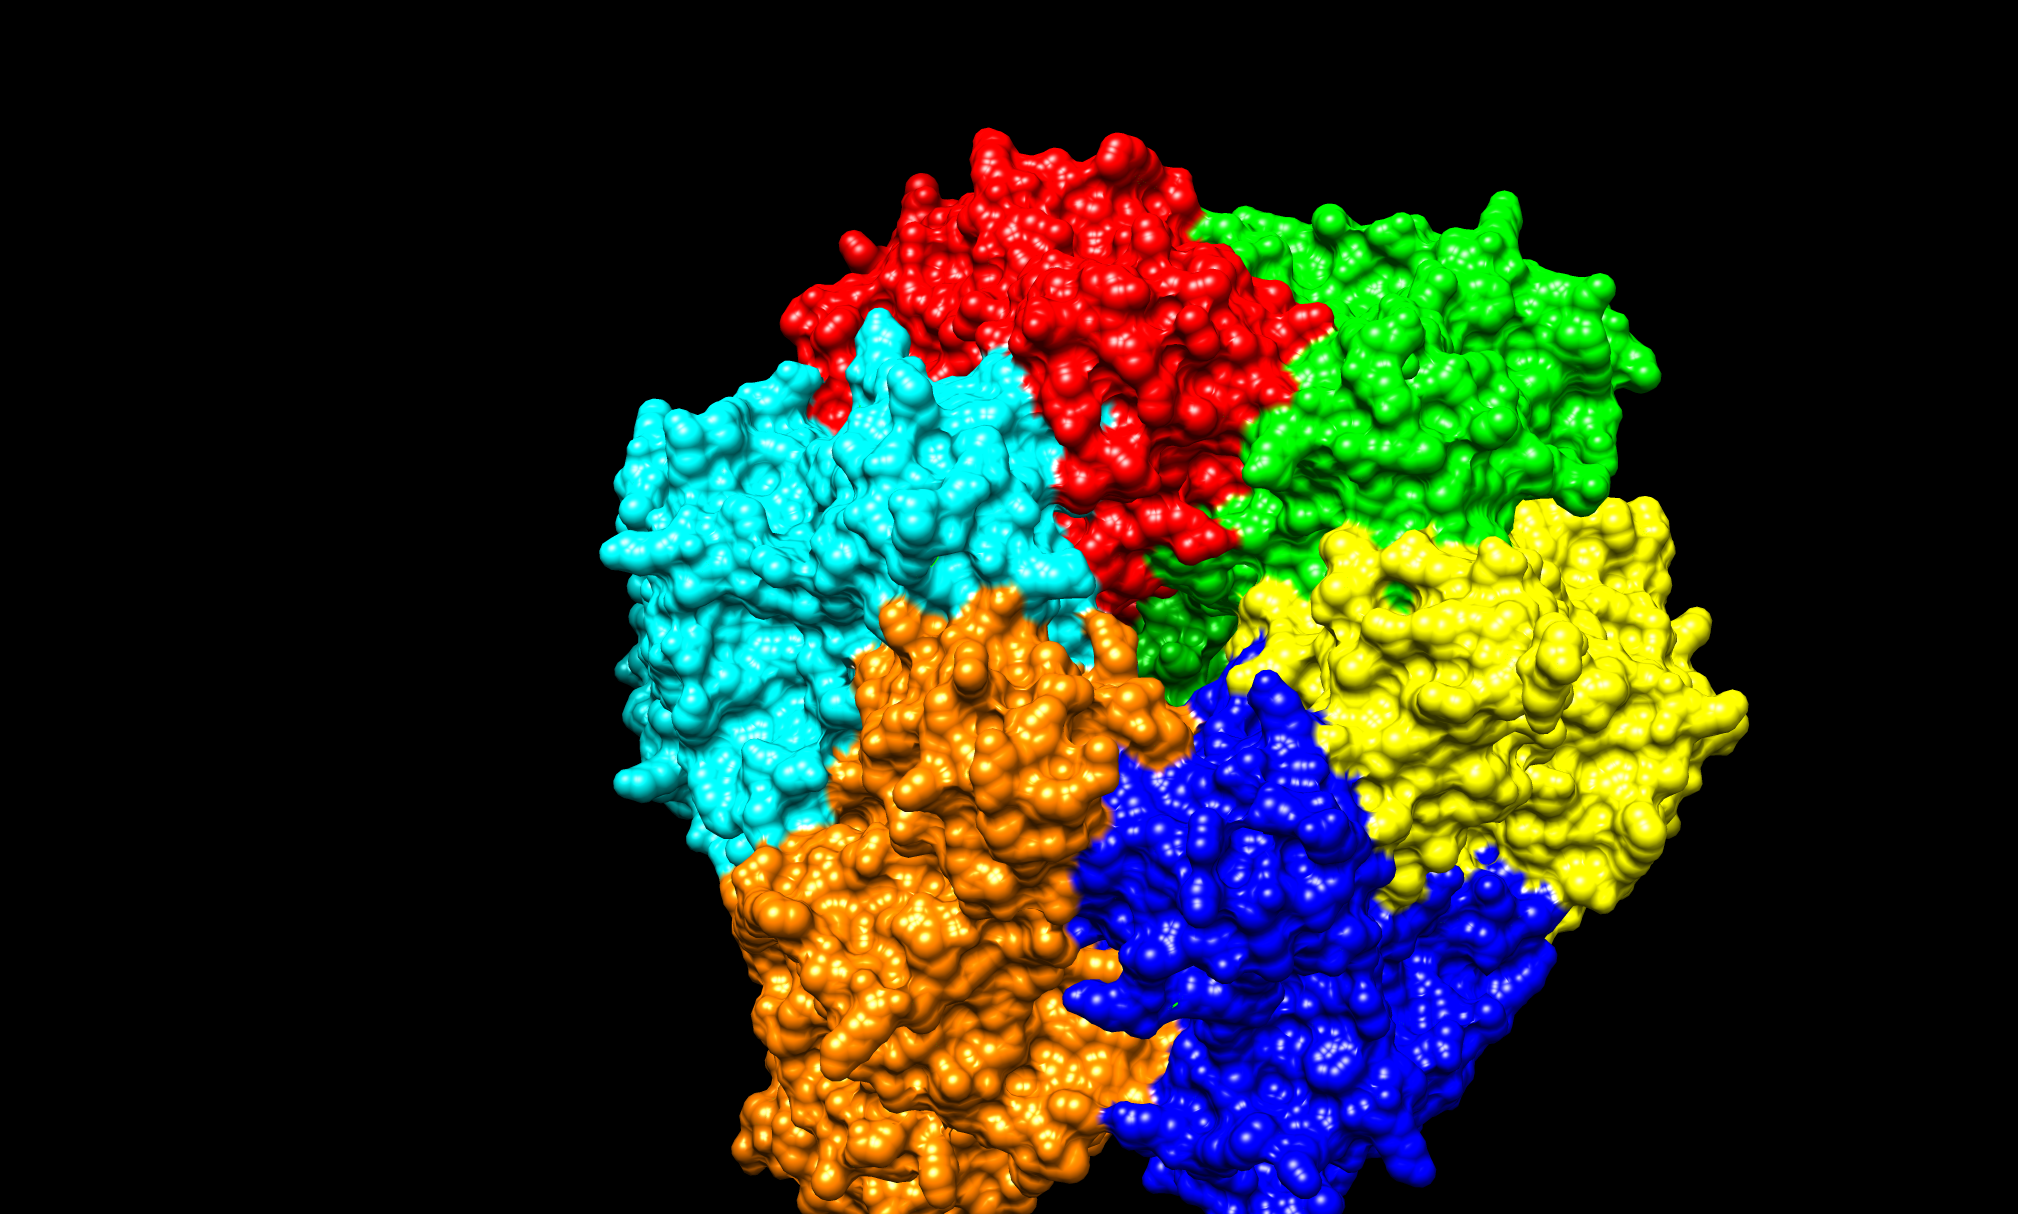
\includegraphics[width=.8\linewidth]{2_h2.png}
    \caption{2.h2}
    \label{fig:2_h2.png}
\end{figure}
\subsection*{(i) Select all the lysines (how many?), color them white and display the side chains}
153 lysines
\begin{figure}[H]
    \centering
    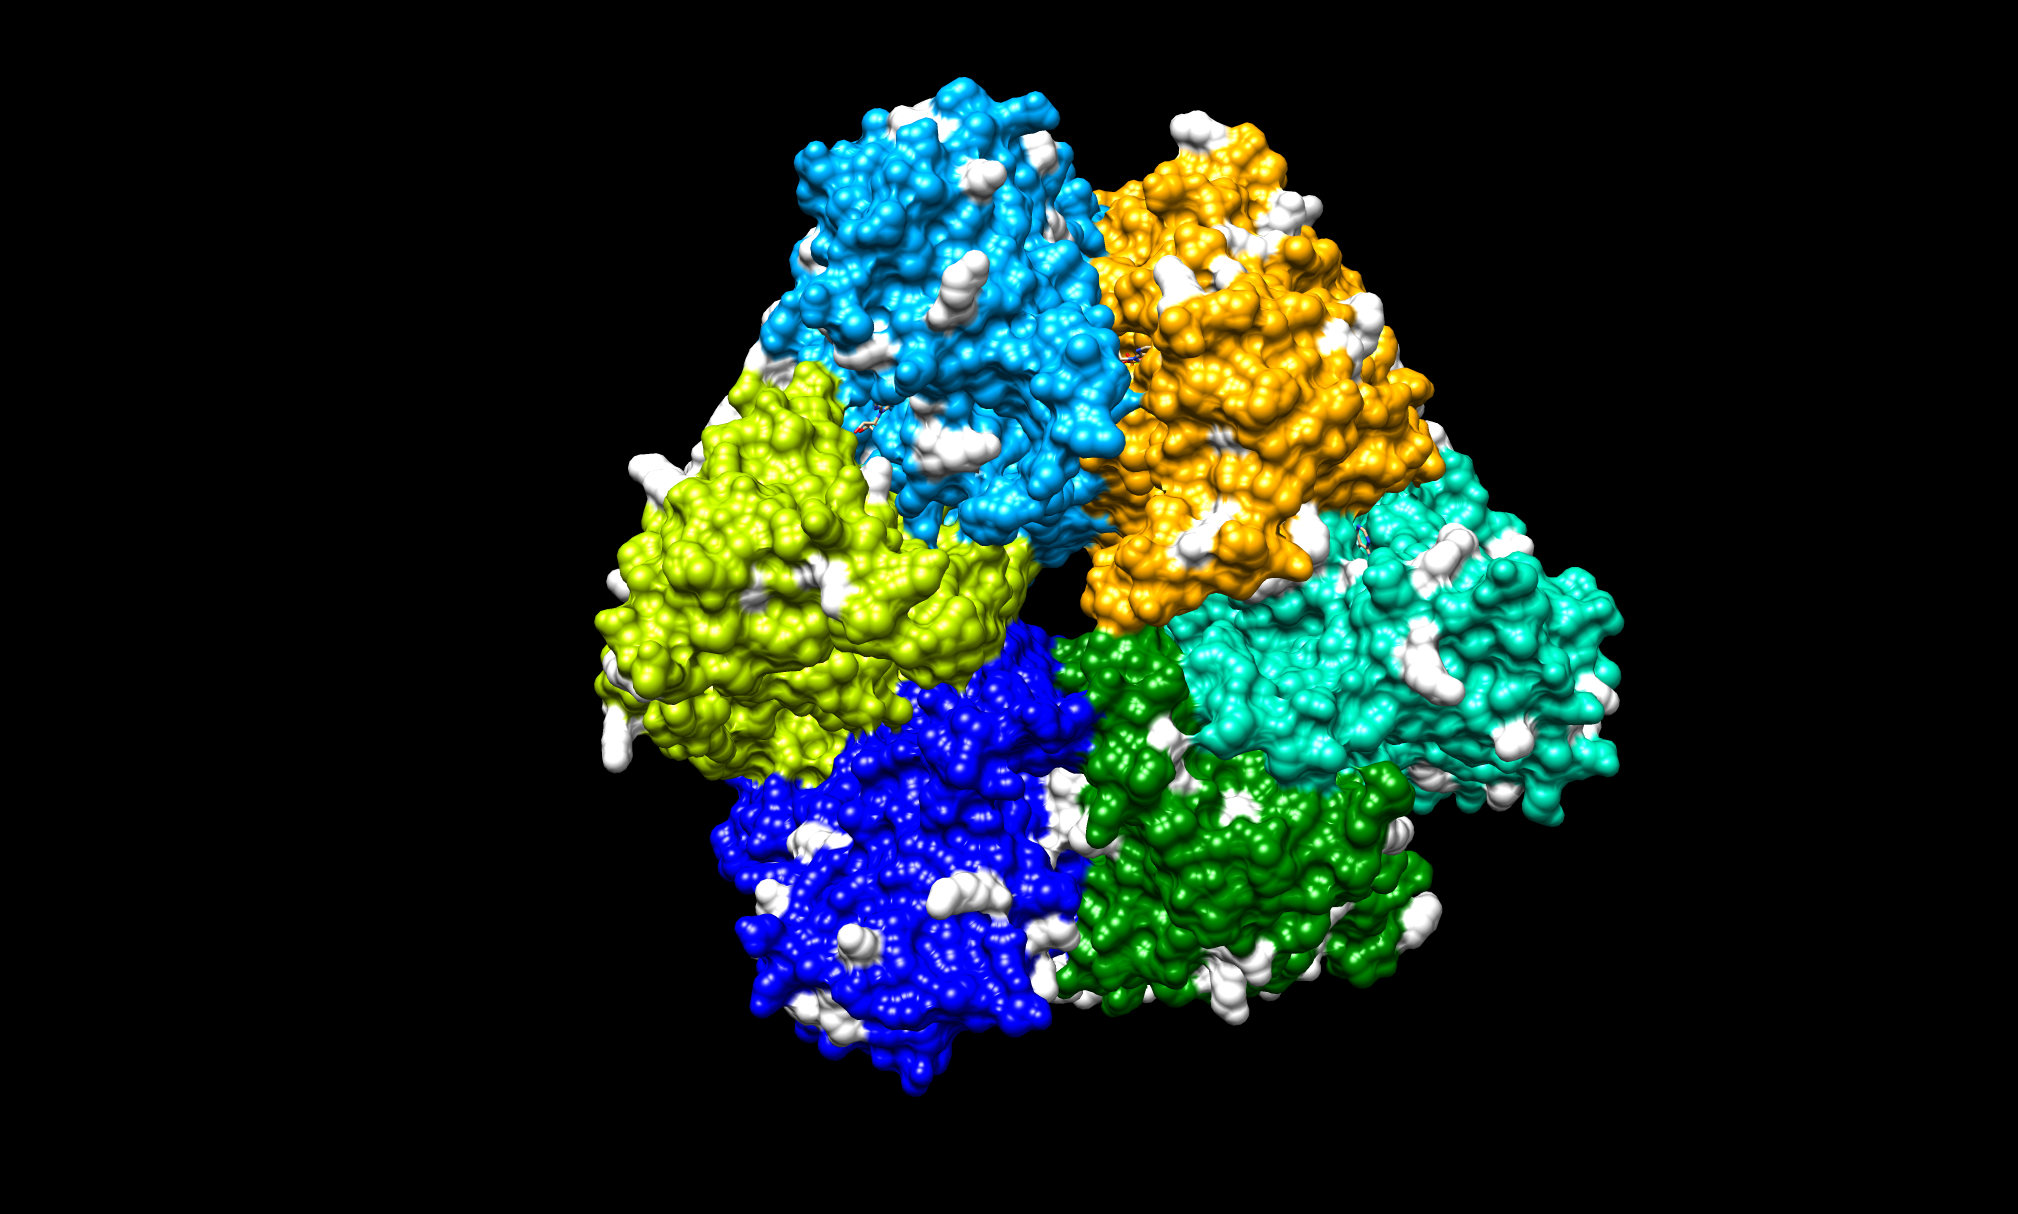
\includegraphics[width=.8\linewidth]{2_i.png}
    \caption{2.i}
    \label{fig:2_i.png}
\end{figure}
\begin{figure}[H]
    \centering
    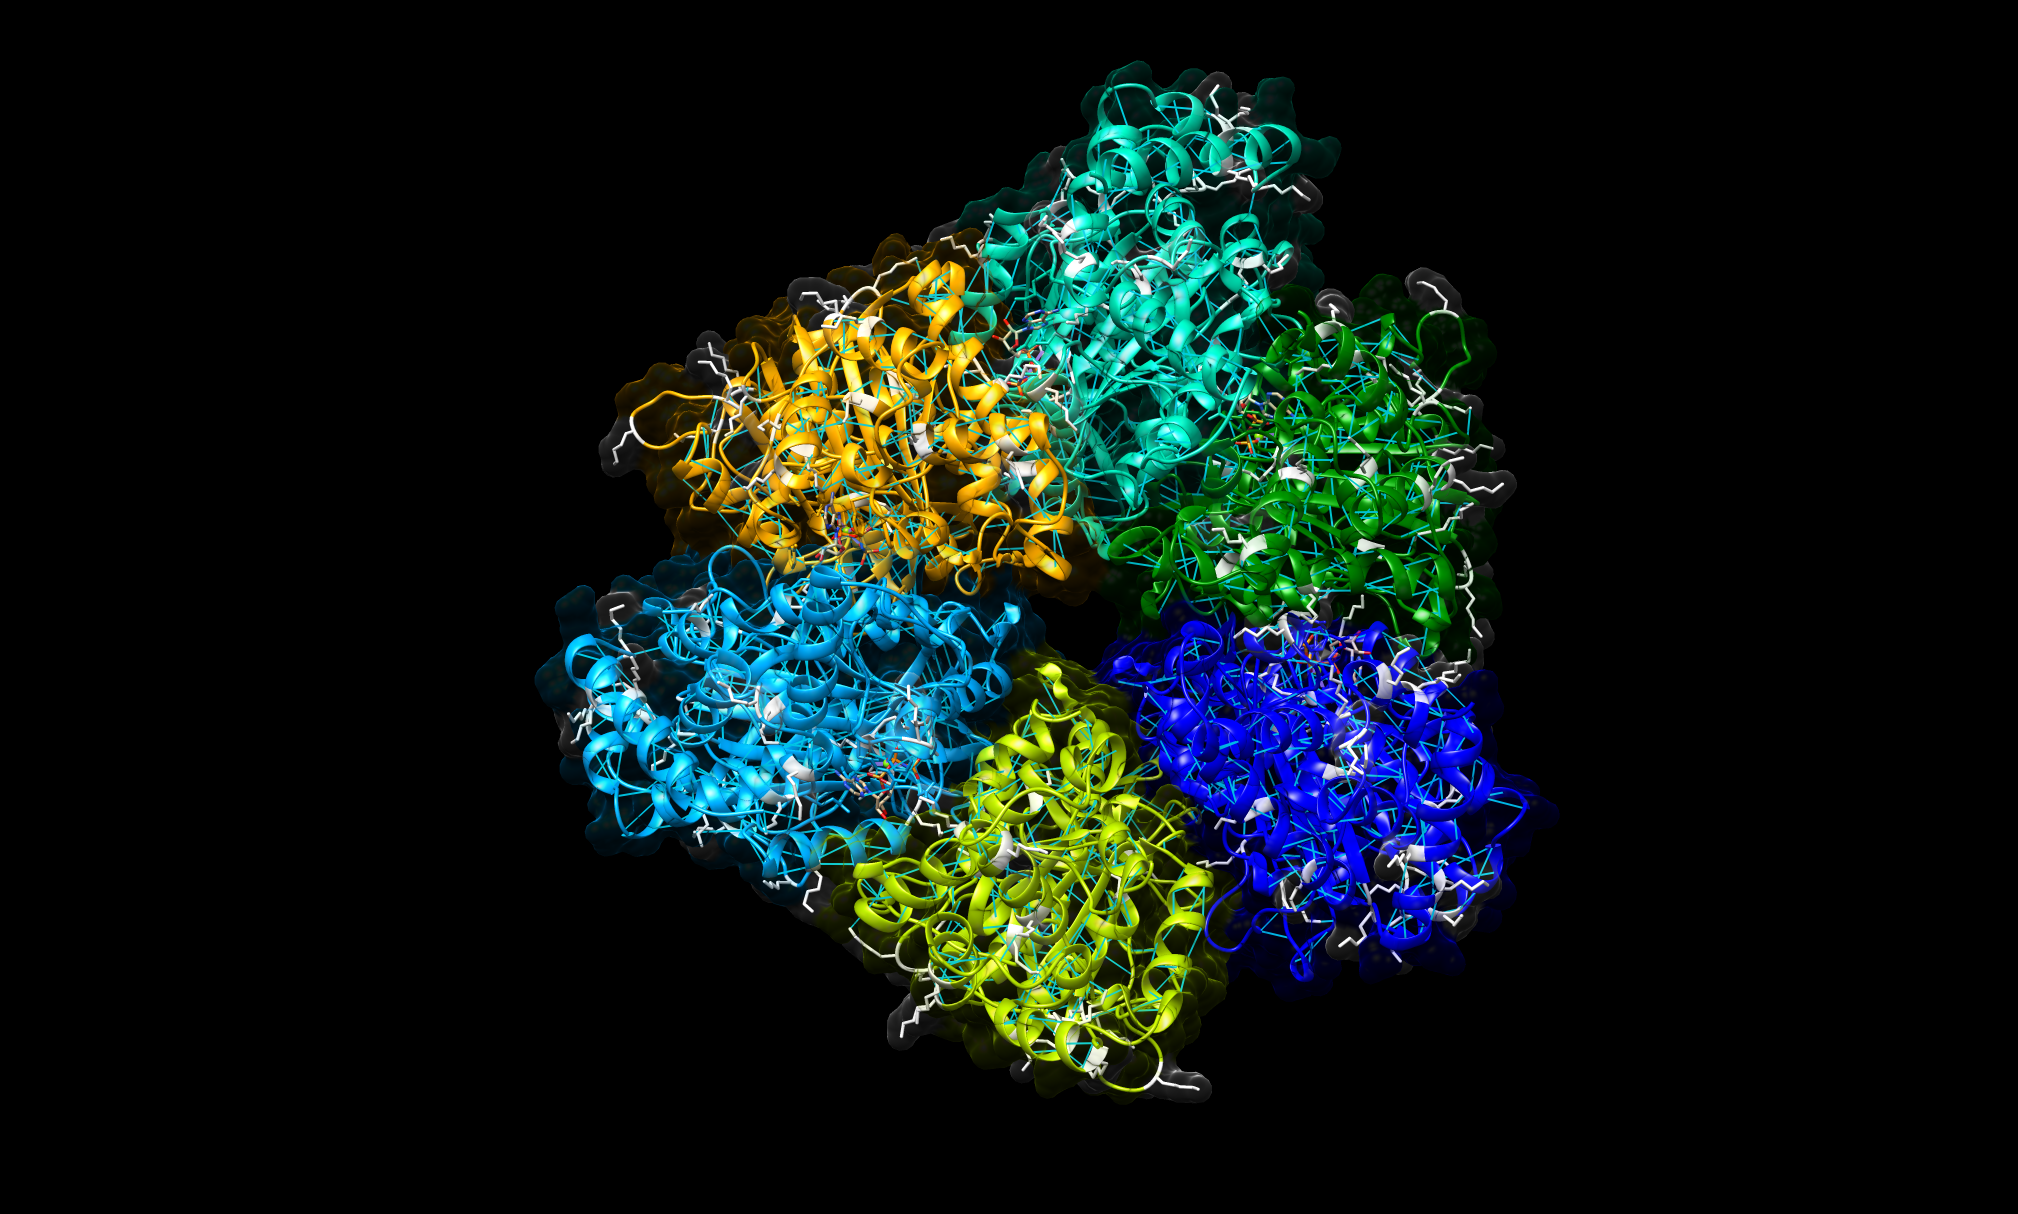
\includegraphics[width=.8\linewidth]{2_i2.png}
    \caption{2.i2}
    \label{fig:2_i2.png}
\end{figure}
\subsection*{(j) Record a video with the rotating structure and join the resulting files.}

\bibliography{refs}
\end{document}